\documentclass[12pt]{llncs}
%\documentclass{jktr}

\usepackage[pdftex]{hyperref}                   
\usepackage {listings}
\usepackage {mathpartir}
\usepackage{bcprules}
%\usepackage{listings}
                       
\usepackage{graphicx} 
%\usepackage[margins=2.5cm,nohead,nofoot]{geometry}
%\usepackage{geometry}
\usepackage{amsfonts}
\usepackage{amstext}
\usepackage{latexsym}
\usepackage{amssymb}
\usepackage{color}


%\include{myPreamble}

% Double brackets
\newcommand{\ldb}{[\![}
\newcommand{\rdb}{]\!]}
\newcommand{\ldrb}{(\!(}
\newcommand{\rdrb}{)\!)}
\newcommand{\lrbb}{(\!|}
\newcommand{\rrbb}{|\!)}
\newcommand{\lliftb}{\langle\!|}
\newcommand{\rliftb}{|\!\rangle}
%\newcommand{\plogp}{:\!-}
\newcommand{\plogp}{\leftarrow}
%\newcommand{\plogp}{\coloneq}
% \newcommand{\lpquote}{\langle}
% \newcommand{\rpquote}{\rangle}
% \newcommand{\lpquote}{\lceil}
% \newcommand{\rpquote}{\rceil}
\newcommand{\lpquote}{\ulcorner}
\newcommand{\rpquote}{\urcorner}
\newcommand{\newkw}{\nu}

% SYNTAX
\newcommand{\id}[1]{\texttt{#1}}
\newcommand{\none}{\emptyset}
\newcommand{\eps}{\epsilon}
\newcommand{\set}[1]{\{#1\}}
\newcommand{\rep}[2]{\id{\{$#1$,$#2$\}}}
\newcommand{\elt}[2]{\id{$#1$[$#2$]}}
\newcommand{\infinity}{$\infty$}

\newcommand{\pzero}{\mathbin{0}}
\newcommand{\seq}{\mathbin{\id{,}}}
\newcommand{\all}{\mathbin{\id{\&}}}
\newcommand{\choice}{\mathbin{\id{|}}}
\newcommand{\altern}{\mathbin{\id{+}}}
\newcommand{\juxtap}{\mathbin{\id{|}}}
\newcommand{\concat}{\mathbin{.}}
\newcommand{\punify}{\mathbin{\id{:=:}}}
\newcommand{\fuse}{\mathbin{\id{=}}}
\newcommand{\scong}{\mathbin{\equiv}}
\newcommand{\nameeq}{\mathbin{\equiv_N}}
\newcommand{\alphaeq}{\mathbin{\equiv_{\alpha}}}
\newcommand{\names}[1]{\mathbin{\mathcal{N}(#1)}}
\newcommand{\freenames}[1]{\mathbin{\mathcal{FN}(#1)}}
\newcommand{\boundnames}[1]{\mathbin{\mathcal{BN}(#1)}}
%\newcommand{\lift}[2]{\texttt{lift} \; #1 \concat #2}
\newcommand{\binpar}[2]{#1 | #2}
\newcommand{\outputp}[2]{#1!(#2)}
\newcommand{\prefix}[3]{#1?(#2) . #3}
\newcommand{\lift}[2]{#1 \lliftb #2 \rliftb}
\newcommand{\clift}[1]{\lliftb #1 \rliftb}
\newcommand{\quotep}[1]{\lpquote #1 \rpquote}
\newcommand{\dropn}[1]{\rpquote #1 \lpquote}
\newcommand{\procn}[1]{\stackrel{\vee}{x}}

\newcommand{\newp}[2]{(\newkw \; #1 ) #2}
\newcommand{\bangp}[1]{! #1}

\newcommand{\substp}[2]{\{ \quotep{#1} / \quotep{#2} \}}
\newcommand{\substn}[2]{\{ #1 / #2 \}}

\newcommand{\psubstp}[2]{\widehat{\substp{#1}{#2}}}
\newcommand{\psubstn}[2]{\widehat{\substn{#1}{#2}}}

\newcommand{\applyp}[2]{#1 \langle #2 \rangle}
\newcommand{\absp}[2]{( #1 ) #2}
\newcommand{\annihilate}[1]{#1^{\times}}
\newcommand{\dualize}[1]{#1^{\bullet}}

\newcommand{\transitions}[3]{\mathbin{#1 \stackrel{#2}{\longrightarrow} #3}}
\newcommand{\meaningof}[1]{\ldb #1 \rdb}
\newcommand{\pmeaningof}[1]{\ldb #1 \rdb}
\newcommand{\nmeaningof}[1]{\lrbb #1 \rrbb}

\newcommand{\Proc}{\mathbin{Proc}}
\newcommand{\QProc}{\quotep{\mathbin{Proc}}}

\newcommand{\entailm}{\mathbin{\vdash_{\mathfrak m}}} %matching
\newcommand{\entailp}{\mathbin{\vdash_{\mathfrak p}}} %behavioral
\newcommand{\entailv}{\mathbin{\vdash_{\mathfrak v}}} %validation
\newcommand{\congd}{\mathbin{\equiv_{\mathfrak d}}}
\newcommand{\congs}{\mathbin{\equiv_{\mathfrak s}}}
\newcommand{\congp}{\mathbin{\equiv_{\mathfrak p}}}
%\newcommand{\logequiv}{\mathbin{\leftrightarrow}}

\newcommand{\barb}[2]{\mathbin{#1 \downarrow_{#2}}}
\newcommand{\dbarb}[2]{\mathbin{#1 \Downarrow_{#2}}}

% From pi-duce paper
\newcommand{\red}{\rightarrow}
\newcommand{\wred}{\Rightarrow}
\newcommand{\redhat}{\hat{\longrightarrow}}
\newcommand{\lred}[1]{\stackrel{#1}{\longrightarrow}} %transitions
\newcommand{\wlred}[1]{\stackrel{#1}{\Longrightarrow}}

\newcommand{\opm}[2]{\overline{#1} [ #2 ]} % monadic
\newcommand{\ipm}[2]{{#1} ( #2 )} 
\newcommand{\ipmv}[2]{{#1} ( #2 )} % monadic
\newcommand{\parop}{\;|\;}		% parallel operator
\newcommand{\patmatch}[3]{#2 \in #3 \Rightarrow #1}
\newcommand{\sdot}{\, . \,}		% Space around '.'
\newcommand{\bang}{!\,}
%\newcommand{\fuse}[1]{\langle #1 \rangle}		
\newcommand{\fusion}[2]{#1 = #2} % fusion prefix/action
\newcommand{\rec}[2]{\mbox{\textsf{rec}} \, #1. \, #2}
\newcommand{\match}[2]{\mbox{\textsf{match}} \; #1 \; \mbox{\textsf{with}} \; #2}
\newcommand{\sep}{:}
\newcommand{\val}[2]{\mbox{\textsf{val}} \; #1 \; \mbox{\textsf{as}} \; #2}

\newcommand{\rel}[1]{\;{\mathcal #1}\;} %relation
\newcommand{\bisim}{\stackrel{.}{\sim}_b} %bisimilar
\newcommand{\wb}{\approx_b} %weak bisimilar
\newcommand{\bbisim}{\stackrel{\centerdot}{\sim}} %barbed bisimilar
\newcommand{\wbbisim}{\stackrel{\centerdot}{\approx}} %weak barbed bisimilar
\newcommand{\bxless}{\lesssim}	%expansion less (amssymb required)
\newcommand{\bxgtr}{\gtrsim}	%expansion greater (amssymb required)
\newcommand{\beq}{\sim}		%barbed congruent
\newcommand{\fwbeq}{\stackrel{\circ}{\approx}}	%weak barbed congruent
\newcommand{\wbeq}{\approx}	%weak barbed congruent
\newcommand{\sheq}{\simeq}	%symbolic hypereq
\newcommand{\wbc}{\approx_{cb}}

% rho logic

\newcommand{\ptrue}{\mathbin{true}}
\newcommand{\psatisfies}[2]{#1 \models #2}
\newcommand{\pdropf}[1]{\rpquote #1 \lpquote}
\newcommand{\plift}[2]{#1 \lliftb #2 \rliftb}
\newcommand{\pprefix}[3]{\langle #1 ? #2 \rangle #3}
\newcommand{\pgfp}[2]{\textsf{rec} \; #1 \mathbin{.} #2}
\newcommand{\pquant}[3]{\forall #1 \mathbin{:} #2 \mathbin{.} #3}
\newcommand{\pquantuntyped}[2]{\forall #1 \mathbin{.} #2}
\newcommand{\riff}{\Leftrightarrow}

\newcommand{\PFormula}{\mathbin{PForm}}
\newcommand{\QFormula}{\mathbin{QForm}}
\newcommand{\PropVar}{\mathbin{\mathcal{V}}}

% qm notation
\newcommand{\state}[1]{\juxtap #1 \rangle}
\newcommand{\event}[1]{\langle #1 \juxtap}
\newcommand{\innerprod}[2]{\langle #1 \juxtap #2 \rangle}
\newcommand{\prmatrix}[2]{\juxtap #1 \rangle \langle #2 \juxtap}
\newcommand{\fprmatrix}[3]{\juxtap #1 \rangle #2 \langle #3 \juxtap}

% End piduce contribution

\newcommand{\typedby}{\mathbin{\:\colon}}
\newcommand{\mixedgroup}[1]{\id{mixed($#1$)}}
\newcommand{\cast}[2]{\id{CAST AS} \; #1 \; (#2)}
\newcommand{\bslsh}{\mathbin{\id{\\}}}
\newcommand{\bslshslsh}{\mathbin{\id{\\\\}}}
\newcommand{\fslsh}{\mathbin{\id{/}}}
\newcommand{\fslshslsh}{\mathbin{\id{//}}}
\newcommand{\bb}[1]{\mbox{#1}}
\newcommand{\bc}{\mathbin{\mathbf{::=}}}
%\newcommand{\bm}{\mathbin{\mathbf\mid}}
\newcommand{\be}{\mathbin{=}}
\newcommand{\bd}{\mathbin{\buildrel {\rm \scriptscriptstyle def} \over \be}}
%\newcommand{\category}[1]{\mbox{\bf #1}}

%GRAMMAR
\newlength{\ltext}
\newlength{\lmath}
\newlength{\cmath}
\newlength{\rmath}
\newlength{\rtext}

\settowidth{\ltext}{complex type name}
\settowidth{\lmath}{$xxx$}
\settowidth{\cmath}{$::=$}
\settowidth{\rmath}{\id{attributeGroup}}
\settowidth{\rtext}{repetition of $g$ between $m$ and $n$ times}

\newenvironment{grammar}{
  \[
  \begin{array}{l@{\quad}rcl@{\quad}l}
  \hspace{\ltext} & \hspace{\lmath} & \hspace{\cmath} & \hspace{\rmath} & \hspace{\rtext} \\
}{
  \end{array}\]
}

% Over-full v-boxes on even pages are due to the \v{c} in author's name
%\vfuzz2pt % Don't report over-full v-boxes if over-edge is small

% THEOREM Environments ---------------------------------------------------
% MATH -------------------------------------------------------------------
 \newcommand{\veps}{\varepsilon}
 \newcommand{\To}{\longrightarrow}
 \newcommand{\h}{\mathcal{H}}
 \newcommand{\s}{\mathcal{S}}
 \newcommand{\A}{\mathcal{A}}
 \newcommand{\J}{\mathcal{J}}
 \newcommand{\M}{\mathcal{M}}
 \newcommand{\W}{\mathcal{W}}
 \newcommand{\X}{\mathcal{X}}
 \newcommand{\BOP}{\mathbf{B}}
 \newcommand{\BH}{\mathbf{B}(\mathcal{H})}
 \newcommand{\KH}{\mathcal{K}(\mathcal{H})}
 \newcommand{\Real}{\mathbb{R}}
 \newcommand{\Complex}{\mathbb{C}}
 \newcommand{\Field}{\mathbb{F}}
 \newcommand{\RPlus}{\Real^{+}}
 \newcommand{\Polar}{\mathcal{P}_{\s}}
 \newcommand{\Poly}{\mathcal{P}(E)}
 \newcommand{\EssD}{\mathcal{D}}
 \newcommand{\Lom}{\mathcal{L}}
 \newcommand{\States}{\mathcal{T}}
 \newcommand{\abs}[1]{\left\vert#1\right\vert}
% \newcommand{\set}[1]{\left\{#1\right\}}
%\newcommand{\seq}[1]{\left<#1\right>}
 \newcommand{\norm}[1]{\left\Vert#1\right\Vert}
 \newcommand{\essnorm}[1]{\norm{#1}_{\ess}}

%%% NAMES
\newcommand{\Names}{{\mathcal N}}
\newcommand{\Channels}{{\sf X}}
\newcommand{\Variables}{{\mathcal V}}
\newcommand{\Enames}{{\mathcal E}}
\newcommand{\Nonterminals}{{\mathcal S}}
\newcommand{\Pnames}{{\mathcal P}}
\newcommand{\Dnames}{{\mathcal D}}
\newcommand{\Types}{{\mathcal T}}

\newcommand{\fcalc}{fusion calculus}
\newcommand{\xcalc}{${\mathfrak x}$-calculus}
\newcommand{\lcalc}{$\lambda$-calculus}
\newcommand{\pic}{$\pi$-calculus}
\newcommand{\spic}{spi-calculus}
\newcommand{\rhoc}{$\rho$-calculus}
\newcommand{\rhol}{$\rho$-logic}
\newcommand{\hcalc}{highwire calculus}
\newcommand{\dcalc}{data calculus}
%XML should be all caps, not small caps. --cb
%\newcommand{\xml}{\textsc{xml}}
\newcommand{\xml}{XML} 
 

%\ifpdf
%\usepackage[pdftex]{graphicx}
%\else
%\usepackage{graphicx}
%\fi

 % \ifpdf
%  \usepackage{pdfsync}
%  \if


%\title{Brief Article}
%\author{David F. Snyder}
%\author{L.G. Meredith}

%\address{Dept. of Math., Texas State University--San Marcos, San Marcos, TX 78666}
       
\pagestyle{empty}


\begin{document}

\lstset{language=[Objective]Caml,frame=shadowbox}

\def\lastname{Meredith}

\title{Notes on interpreting quantum mechanics in a reflective process calculus}
\titlerunning{quantum processes}

\author{ L.G. Meredith\inst{1} }
\institute{ Partner, Biosimilarity\\ 505 N72nd St, Seattle, WA 98103, USA, \\
  \email{ lgreg.meredith@biosimilarity.com } 
} 

\maketitle              % typeset the title of the contribution

%%% ----------------------------------------------------------------------

\begin{abstract}

  We sketch an interpretation of operations of quantum mechanics in
  terms of operations in a reflective process calculus.

\end{abstract}

%\keywords{Process calculi, knots, invariants}

% \begin{keyword}
% concurrency, message-passing, process calculus, reflection, program logic
% \end{keyword}

%\end{frontmatter}

% section front matter (end)

\section{Introduction}\label{sec:introduction} % (fold)
For the past several centuries there has been no serious competitor to
the ``Newtonian'' account of dynamics in the physical sciences. Here
we mean the mathematical apparati of the integral and derivative and
the principles of applications of those apparati to modeling dynamical
systems, such as the Lagrangian and Hamiltonian \cite{375178}. As a
result the predominant share of accounts of dynamical systems and
situations have had to be formulated in terms of the Newtonian
machinery. The present author views this as an intellectually
dangerous position to occupy. Everything, despite it's intrinsic
shape, turns into a nail to be hit with this hammer. For example, even
challenges to classical accounts of physics as deep as General
Relativity \cite{Gravitation} and Quantum mechanics \cite{Dirac1930}
are still \emph{essentially} couched in the methods and procedures
derived from the Newtonian integral and derivative \footnote{The
  covariant derivative still bears the imprimature of the original
  notion. Inner product in the wave-function formulation is still an
  integral}. Recently, however, the theory of computation has matured
to the point where we have candidates for theories of dynamics that
offer very different perspectives on reasoning about dynamical systems
and situations. It is time to see just how good they are by addressing
the dynamics of interest in the physical sciences. Testing these
candidates against very successful accounts of dynamical situations,
like quantum mechanics, is going to give us some sense of maturity,
quality and range of applicability of computational notions of
dynamics.

To address this program we realize and carry out the calculations of
quantum mechanics over a novel formal theory of dynamics, a formal
theory of dynamics that corresponds to a theory of concurrent
computation with \emph{reflection}
\cite{bcsmith:phdthesis},\cite{319871}. It has the advantage that the
underlying theory is already `quantized', but supports analogues all
of the continuuous operations. Strikingly, this underlying theory has
recently been connected with a notion of metric
\cite{DBLP:conf/fossacs/BreugelMOW03} that coincides with the metric
induced by the inner product.

\subsection{Summary of contributions and outline of paper}

The plan is to develop an interpretation of the operations of quantum
mechanics normally interpreted by Hilbert spaces and operators
\cite{MathematicalFoundationsQM}. The primary novelty of the approach
is to do this over a theory of computation. Note that this is very
different than the usual quantum computation program which develops
notions of computation over quantum mechanics \cite{544199}. Rather,
we are developing a story that aligns with Wheeler's slogan: It from
Bit \cite{HowComeTime}. To do this we will first provide an account of
the theory of computation at play here. Then we will dive into a
calculation-driven interpretation of the operations of quantum
mechanics.

The reason we take this approach is that -- until very recently
(\cite{DBLP:conf/lics/Abramsky04},
\cite{DBLP:conf/calco/Abramsky05})-- there hasn't been an axiomatic
account of quantum mechanics. As a result there has been no sharp
delineation of the mathematical theory supporting interpretation of
the physical theory and the physical theory, itself. So, ambient
features of the maths are free to be exploited (or suppressed) without
a real accounting of their physical relevance. There is no sharp
statement ``here's the physical theory'' qua \emph{theory} and
``here's the mathematical interpretation'' enabling a judgment of how
faithful the interpretation is -- apart from experimental
observation. When there is an axiomatic account we can judge how well
a given mathematical formalism supports an interpretation of the
axioms, independent of experimentation. Likewise, we can judge how
well we have captured our physical evidence and experience with our
axiomatics, independent of any specific mathematical implementation,
with accidental detail that may or may not have physical significance.

In lieu of a fully fleshed out and vetted axiomatic account of quantum
mechanics, interpreting the operational notions in service of modeling
physical systems will have to suffice. In other words, we are not in
the business of providing a model of Hilbert spaces and operators. We
are in the business of providing a model of quantum mechanics because
we are motivated by testing our notions of dynamics against physical
theory; and, the predictive calculations of the physical theory must
serve as the best formulation -- shy of a fully fleshed out axiomatic
account -- of the physical theory itself (as they have for scientific
theories since time immemorial). Put another way, despite a
whole-hearted commitment to an It-from-Bit ontology, we are firmly
aligned with the shut-up-and-calculate camp as the best way to obtain
results either from the physical perspective or as a quality assurance
measure of our fledgling theory of dynamics.

In detail, we present a reflective process calculus. Then we develop
intuitive correspondences between the notions available in this
calculus and the usual physical notions supporting quantum mechanical
calculations. 

\begin{table}[htp]
  \center{
    \fbox{
      \begin{tabular}{c|c}
        quantum mechanics & process calculus \\
        \hline
        scalar & name \\
        state vector & process \\
        dual & contextual duals \\
        matrix & formal sums of process-context-dual pairs \\
        orthogonality & process annihilation \\
        inner product & execution-formula + quoting
      \end{tabular}
    }
  }
  \caption{QM - process calculi correspondences}
\end{table}

Then we tighten up these intuitions to operational definitions. We
employ the Dirac notation as the best proxy we can find for an
abstract syntax of the quantum mechanical notions. The definitions we
develop put us in contact with equational constraints coming from the
theory that we demonstrate the definitions and calculations satisfy.

This puts us in a position to shut up and calculate for the
Stern-Gerlach experimental set up, showing how these predictive
calculations become calculations on processes in our theory of a
reflective process calculus. The particular example is of interest
because it is a composite experiment, consisting of iterated
measurements. The framework developed here is particularly suited to
reasoning about composite physical systems and situations.

Penultimately, we demonstrate that the notion of metric coming from
the inner product coincides with the notion of metric available from
the theory of bisimulation. This demonstration gives us the right to
think of space as arising from behavior. Finally, we consider where we
might go from the new vantage point we have obtained.

% section introduction (end) 
 
% section introduction (end)

% \section{A summary of knot presentations}\label{sec:notation} % (fold)


The knot presentations we focus upon herein are the Gauss code \cite{Read1977On-the-Gauss-cr}, the
Dowker-Thistle\-thwaite (DT) code \cite{DT}, the Conway notation \cite{Conway1970An-enumeration-}, and the Master
Code of Rankin, Schermann and Smith \cite{Rankin2004Enumerating-I} \cite{Rankin2004Enumerating-II}. Other presentation schemes, such
as braid representatives and Morse links, are not directly useful to
the development of this paper and thus are overlooked. We also give a
``wish-list'' of properties one would desire from one's knot notation
scheme.

\subsection{Knot presentations}
This section briefly discusses various knot notations and establishes
some terminology, with references for readers needing further details.

\subsubsection{Regular knot projections}

In 1847, J.B. Listing classified knots up to 5 crossings by analyzing
knot projections \cite{Listing1848Vorstudien-zur-}. Listing was the
first to publish an article containing a drawing of a regular knot
projection (or \emph{knot diagram} or \emph{planar diagram}). A
\emph{knot} is taken to be a polygonal simple closed curve in
$3$-space. Choose any plane on which projection onto the plane results
in a curve whose only singularities are transverse double points which
are not the image of any vertex from the polygonal curve. Using a
canonical normal vector to the plane for line of sight, for a given
double point $d$ we find the point $c$ in the projection's preimage of
$d$ farthest from our line of sight, and we indicate an undercrossing
by erasing the image of a small neighborhood of $c$ from the planar
projection. A careful presentation is given in \cite{LivingstonText}.
	
Out of all possible regular projections of a knot, there is (at least)
one with minimal number of crossings. 

% We'll write $\#(K)$ to denote this number.


\subsubsection{The Gauss code.} Gauss used regular knot projections to
arrive at what is now called the Gauss Code of a knot
\cite{Read1977On-the-Gauss-cr}. The Gauss code is the first knot notation
system. P. G. Tait used an encoding in the 1870's to classify knots up
to 7 crossings \cite{Tait}. Tait's encoding may be regarded as an
extension to the Gauss Code. One begins somewhere on the knot
projection (not at a crossing point), then proceeds along the knot
applying labels to the first, third, fifth etc. crossing until all
crossings are labeled; one then traverses the knot once more, writing
the label of each crossing in the order that you reach it, attaching a
plus or minus sign, depending on whether you are crossing over or
under.

\subsubsection{Tait, Little, and Kirkman.} Using Kirkman's
classification of certain polygons \cite{Kirkman1885The-enumeration},
Tait (and Little, using similar methods) was able to tabulate knots up
to 11 crossings \cite{Tait} \cite{Little1885On-knots-with-a}
\cite{Little1890Alternate-pm-kn}
\cite{Little1900Non-alternate-p}. Tait's system included using a
simple reduction rewrite strategy within his notation system. This notation was improved by Dowker and Thistlethwaite, as discussed in some detail below.



\subsubsection{Reidemeister moves.} Reidemeister developed a reduction
rewrite system for knot projections (“the three Reidemeister moves”)
\cite{ReidemeisterMoves}. We illustrate the three moves. The
convention in these (and in other graphically-based invariants) is
that we show only the relevant part of the knot. In our diagrams here,
we have placed dashed circles, which the reader should imagine as
viewing through scope lens only a portion of the knot, with
the remainder of the knot outside of the scope of view and unchanged.

\begin{figure}[hbt]
    \centering
    \scalebox{0.37}[0.370]{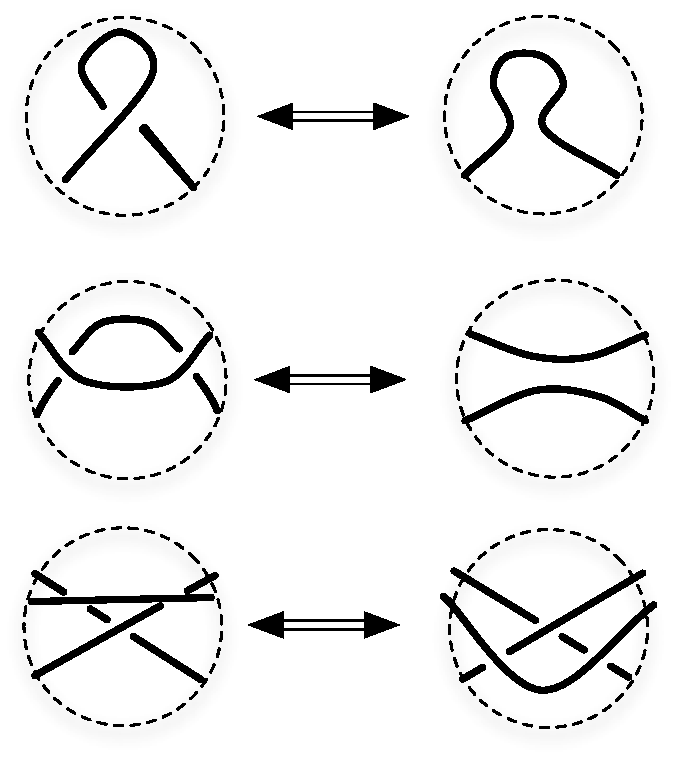
\includegraphics[viewport=0 0 390 360]{../../illustrations/Reidemeister123vert.pdf}}
    \caption{ The three Reidemeister moves. The topmost move will be referred to as $R_1$, the middle one as $R_2$, and the bottommost as $R_3$. For any one of these moves $R$, we write $R^{\to}(K)$ (resp. $R^\leftarrow$(K)) if the move has been applied left-to-right (resp. right-to-left)  to the knot diagram $K$.}
\label{fig:RMoves}
\end{figure}

The import of this system is Reidemeister's Theorem: an ambient
isotopy of two knots may be exhibited as sequences of rewrites of (any of) their
diagrams, and vice versa. That is, two knots are ambient isotopic if and only if a
diagram of one may be rewritten, via a sequence of Reidemeister
moves, to a diagram of the other \cite{LivingstonText}.



\subsubsection{Knotation} Conway developed a clever notational system
for tangles, finding an algebraic-like system for this system that led to several methods of reduction rewrites
\cite{Conway1970An-enumeration-}. He used this system to retabulate
knots and links of 11 crossings by hand, in one afternoon (an effort
that took Tait and Little years of work), discovering one omission and
a few duplications in the process. Conway's system can be used to
classify all arithmetic (also called algebraic, or rational)
knots. The Conway code for a knot originally was given as a “basic
polyhedron” followed by a sorted list of arithmetic tangles. See
Conway's paper \cite{Conway1970An-enumeration-} for details. This system has extensions by Caudron
\cite{Caudron1981-Classification} and by Bangert
\cite{Bangert2002Algorithmic-Pro}. Conway has investigated further
structures such as bangles and bracelets.

\subsubsection{Dowker-Thistlethwaite Codes (DT codes)}\label{ssub:dowker_thistlethwaite_codes} % (fold)
Dowker created a variation of Tait's notational system that is easier
to implement computationally. Dowker and Thistlethwaite made it the
basis for an algorithm that successfully enumerated knots of up to 13
crossings \cite{DT}. Not every DT code is valid, i.e. an arbitrary DT
code may not correspond to an actual knot, and two distinct composite
knots may share the same DT Code. However, a valid DT code for a prime
knot specifies the knot uniquely \cite{SchareinPhD}. In their paper,
Dowker and Thistlethwaite develop an algorithm to filter out invalid
cases. They also give a reduction system to remove duplicates from
their enumeration.

We now recall the definition of the DT code of
a regular knot projection \cite{DT}. Begin at a selected point on the
diagram (excepting crossing points) and traverse the diagram in a
selected direction. At each encounter of a crossing, label the
crossing with the next available counting number; for an even label,
prepend a negative sign if traversing the overcross. Returning to the
beginning point, each crossing has been labeled twice, once with an
odd number and once with an even number. Let $S_\pm$ denote the set of
labels generated.

If the knot projection has $n$ crossings, then there are $2n$ labels
(from $1$ to $2n$ in absolute value) and at each crossing an unique
odd counting number paired with an even integer. This induces a
parity-reversing function $\sigma$ on $S= \{1,\ldots,2n\}$, where for
each $i\in S$ we find the crossing with label whose absolute value is $i$ and let
$\sigma(i)$ be the absolute value of the other label at that crossing.
Note that $\sigma(\sigma(i))=i$ for any $i\in S$. Note that there is
also a bijective translation $\tau: S\to S_\pm$ where
$\abs{\tau(s)}=s$ for all $s\in S$.  Then the DT code of the knot
projection is determined by $\delta=\tau\circ\sigma$, usually given as
the list $\{\delta(1),\delta(3),\ldots,\delta(2n-1)\}$. Note that
$\delta\circ\sigma=\tau$. Finally, for each $i\in S$, let $sgn(i)$
denote the sign of $\tau(i)$ (so $sgn(i)<0$ implies $i$ is even).

For each $i\in S_\pm$, let $C(i)$ denote the crossing with label
$i$. Then for any $i\in S$ we know $C(i)$ is adjacent to the two
crossings $C(i\pm 1)$ and $C(\delta(i)\pm 1))$, where addition is modulo $2n$. This fact is applied
later when giving an explicit algorithm for encoding a knot.


% subsubsection dowker_thistlethwaite_codes (end)
 
\subsubsection{From Calvo to Rankin, Flint, and Schermann} Calvo
developed an inductive knot tabulation algorithm, thereby sidestepping the need to
check validity of DT codes \cite{Calvo1997Knot-enumeratio}. However, detection of
duplication within the tables generated then becomes the issue. Calvo had the insight that
understanding the deeper flype structure of prime, non-alternating
diagram led to greater efficiencies in his algorithm. The Calvo
algorithm was essentially refined in the development of a notational
system by Rankin, Flint, and Schermann , based on what they call
the group code which reminds one somewhat of the Gauss code but, instead, using a
Conway-like insertion scheme to allow for easy reduction of flype
structures in the notation \cite{Rankin2004Enumerating-I}
\cite{Rankin2004Enumerating-II} \cite{Rankin2004EnumeratingLinks}. This results in a master array that provides a unique identifier for  prime alternating knots. This forms part of the basis for inductive construction of all prime alternating knots of crossing size $n$ from those of crossing size $n-1$(see the above papers for details).  Composite knots remain problematic, due principally to the issue of detection of duplicates.




\subsection{Desirable properties for a knot presentation system }\label{sub:desirable_properties_for_a_knot_notation_system_} % (fold)

In this section, we list some properties that one would wish for a
knot presentation system to enjoy, followed by a discussion of the
knot presentations of the last subsection in the light of these
wishes.

Due to complexity considerations, one may well despair of a knot
notation system that would allow for mathematical classification of
all knots. However, in designing a system of knot notation or
presentation, informed by the history of knot tabulation and
classification we can enumerate the following properties such a
notation system may enjoy. These properties invariably correspond to
demands of functoriality on the encoding when considered as a map from
the category of knots or braids to some suitable target category while
others are demands on the faithfulness (respectively, fullness) of the
encoding considered as functor.

\begin{itemize}


\item {Surjection (realizability).} Each code in the notation represents
  a knot (or if this is not the case, those codes that do not
  represent a knot are easily recognizable). A code for a knot should
  be easily obtained from one of its planar diagrams.

%\item [Reduction] 
\item {Reduction.} The notation enjoys a calculus with which to reduce
  and simplify encodings. Each step of simplification or reduction
  results in an encoding representing a knot isotopy equivalent to the
  originating knot.

%\item [Minimality] 
\item {Minimality.} The notational encoding of a given knot can be
  reduced to a (finite non-empty set of equivalent) minimal
  encoding(s).

%\item [Injection] 
\item {Well-definedness.} If a knot has two (or more) minimal reduced
  encodings, each of these encodings is equivalent to the notation for
  a knot equivalent \emph{via} ambient isotopy to the original.

\item {Injection.} Two knots that have equivalent
  minimal reduced encodings are ambient isotopic.


	\item {Economy.} The notation is computationally cheap and easily constructed from a diagram of the knot or from a simple code, such as the DT code.
	
%\item [Compositionality] 
\item {Compositionality.} Operations on knots, e.g. knot
  composition, correspond to natural operations on elements in the
  image of the encoding.
  
%\item [Separation] 
\item {Separation.} The notation can be used to classify a class X of
  knots, where X contains a previously classified class of knots (for
  example, arithmetic knots (also known as algebraic knots) and
  bracelets) but is not previously classified itself.

%\item [Classification] 
\item {Extensibility.} The notation enjoys a formal language in which
  to describe properties and invariants of notation objects that
  reflect interesting properties of knots. This language should also
  be useful in selecting specific sets of knots (such as the set of
  all 21-crossing prime alternating links containing the tangle
  5/3). This language ideally should be scaleable and be applicable to
  tables of indefinite size.
\end{itemize}

The DT code, with proper care taken, satisfies the
first six properties but breaks under compositionality. Conway's
tangle notation enjoys all of the properties listed, though the Conway
encoding requires foreknowledge of the classes of basic polygons with
$n$ vertices. The master array of Rankin, Flint, and Schermann 
satisfies the first five properties, but appears unlikely to support
the last four properties to a degree useful for anything other than
tabulation.

\subsubsection{A meta-knotation}

 Due to Reidemeister's Theorem, in order to establish our main theorem we need only consider diagrams of knots and not knots themselves. Hence we  adopt the following convenient
notation and terminology. The meta-variable  $K$
ranges over knot diagrams and we reserve $\mathcal{K}$ to range over knots. For simplicity, we refer to $K$ as a knot. We write $\#(K)$ to mean the number of crossing points in the diagram $K$ but will call this value the crossing number of the knot $K$, which the reader is asked not to confuse with the minimal crossing number of the knot (it is in this sense that we will later say that ``two knots from the same isotopy class can have different crossing numbers'').   Formally speaking $\sim_{\text{iso}}$ will denote  equivalence of knots under ambient
isotopy and $\sim_{R}$ will denote equivalence of diagrams under (finite) sequences of
Reidemeister transforms. However, when there is little chance of confusion we
drop the subscript and write $\sim$.  

% subsection desirable_properties_for_a_knot_notation_system_ (end)

% section notation (end) 

% section notation (end)

\section{Concurrent process calculi and spatial logics }\label{sec:concurrent_process_calculi_and_spatial_logics_} % (fold)
In the last thirty years the process calculi have matured into a
remarkably powerful analytic tool for reasoning about concurrent and
distributed systems. Process-calculus-based algebraical specification of
processes began with Milner's Calculus for Communicating Systems (CCS)
\cite{MilnerCCS80} and Hoare's Communicating Sequential Processes
(CSP) \cite{CSP} \cite{CSP1} \cite{CSP2} \cite{CSP3}, and continue
through the development of the so-called mobile process calculi,
e.g. Milner, Parrow and Walker's $\pi$-calculus \cite{ParrowWalker},
Cardelli and Caires's spatial logic \cite{CairesC04} \cite{CairesC03}
\cite{Caires04}, or Meredith and Radestock's reflective calculi
\cite{MeredithR05} \cite{meredith2005rho}. The process-calculus-based
algebraical specification of processes has expanded its scope of
applicability to include the specification, analysis, simulation and
execution of processes in domains such as:

\begin{itemize}
\item telecommunications, networking, security and application level protocols
\cite{AbadiB02} 
\cite{AbadiB03} 
\cite{BrownLM05} 
\cite{LaneveZ05}; 
\item programming language semantics and design
\cite{BrownLM05}
\cite{djoin}
\cite{JoCaml}
\cite{WojciechowskiS99};
\item webservices
\cite{BrownLM05}
\cite{LaneveZ05}
\cite{MeredithB03};
\item and biological systems
\cite{Cardelli04}
\cite{DanosL03}
\cite{RegevS03}
\cite{PriamiRSS01}.
\end{itemize}

Among the many reasons for the continued success of this approach are
two central points. First, the process algebras provide a
compositional approach to the specification, analysis and execution of
concurrent and distributed systems. Owing to Milner's original
insights into computation as interaction \cite{Milner93}, the process
calculi are so organized that the behavior ---the semantics--- of a
system may be composed from the behavior of its components
\cite{Fokkink}. This means that specifications can be constructed in
terms of components ---without a global view of the system--- and
assembled into increasingly complete descriptions.

The second central point is that process algebras have a potent proof
principle, yielding a wide range of effective and novel proof
techniques \cite{MilnerS92} \cite{SangiorgiWalker} \cite{Sangiorgi95}
\cite{hop}. In particular, \emph{bisimulation} encapsulates an effective
notion of process equivalence that has been used in applications as
far-ranging as algorithmic games semantics
\cite{Abramsky2005Algorithmic-Gam} and the construction of
model-checkers \cite{Caires04}. The essential notion can be stated in
an intuitively recursive formulation: a \emph{bisimulation} between two
processes $P$ and $Q$ is an equivalence relation $E$ relating $P$
and $Q$ such that: whatever action of $P$ can be observed, taking it
to a new state $P'$, can be observed of $Q$, taking it to a new state
$Q'$, such that $P'$ is related to $Q'$ by $E$ and vice versa. $P$ and
$Q$ are \emph{bisimilar} if there is some bisimulation relating
them. Part of what makes this notion so robust and widely applicable
is that it is parameterized in the actions observable of processes
$P$ and $Q$, thus providing a framework for a broad range of
equivalences and up-to techniques \cite{milner92techniques} all governed by the same core
principle \cite{SangiorgiWalker} \cite{Sangiorgi95} \cite{hop}.
% section concurrent_process_calculi_and_spatial_logics_ (end) 

% section concurrent_process_calculi_and_spatial_logics_ (end)
    
%\section{Knots as processes}\label{sec:knots_as_processes} % (fold)

This section bootstraps intuitions about the target calculus by
introducing process expressions for key aspects of a knot's
structure. An $n$ crossing knot $K$ is modeled as a system
$\meaningof{K}$ of concurrently executing processes. More
specifically, $\meaningof{K}$ is a \emph{parallel composition} $\Pi_{i
  = 0}^{n-1} \meaningof{C(i)} | W$ of $n+1$ processes consisting of
$n$ crossing processes $\meaningof{C(i)}$ and a process $W$
constituting a ``wiring harness.'' The latter process can be thought
of as the computational equivalent to Conway's ``basic polygon,'' if
the knot is in minimal crossing number form. The complete expression
of the encoding is

% \begin{eqnarray*}
%   \meaningof{K} & := &  (v_0 ... v_{4n-1})( \Pi_{i = 0}^{n-1} (\nu \; u)\meaningof{C(i)}(v_{4i},...,v_{4i+3},u) \\
%   & & \; \; \; \; \; \; \; \; \; \; \; \; \; \; \; \; \; \; | \Pi_{i = 0}^{n-1} W(v_{\omega(i,0)},v_{\omega(i,1)})|W(v_{\omega(i,2)},v_{\omega(i,3)}) ) \nonumber
% \end{eqnarray*}

\begin{align*}
  \meaningof{K} :=  (v_0 ... v_{4n-1}) & ( \Pi_{i = 0}^{n-1} (\nu \; u)\meaningof{C(i)}(v_{4i},...,v_{4i+3},u) \\
  & | \Pi_{i = 0}^{n-1} W(v_{\omega(i,0)},v_{\omega(i,1)})|W(v_{\omega(i,2)},v_{\omega(i,3)}) )
\end{align*}

Here, $C(i)$ represents the $i$th crossing in the knot diagram $K$.  The wiring process, $\Pi_{i =
  0}^{n-1}W(v_{\omega(i,0)},v_{\omega(i,1)})|W(v_{\omega(i,2)},v_{\omega(i,3)})$,
is itself a parallel composition of wire processes that correspond to
edges in the 4-valent graph of the knot shadow \cite{SchareinPhD} the constraints of
which are reflected in the indexing function $\omega$. The wiring process
may be calculated from other knot notations. For example,  we later show how the indexing function $\omega$ may be calculated
from $\delta$, the DT code of the knot projection. The crossing and wire
processes have further substructure, outlined below.

\begin{remark}[knots as abstractions]
  The reader familiar with process calculi will observe that the
  encoding actually produces an \emph{abstraction} \cite{SangiorgiWalker}  in $4\#(K)$ names
  (see the first choice in the production labeled agent in the grammar
  of \ref{sub:the_syntax_and_semantics_of_the_notation_system}). This is actually a way of demarking that the encoding should
  be insensitive to the particular set of names chosen to represent the
  ports of the crossings. Some caution must be exercised, however, as
  the encoding only preserves knot structure if the abstraction is
  applied to a vector of $4\#(K)$ distinct names.
\end{remark}

\subsection{Crossing processes}\label{sub:crossing_processes} % (fold)
A crossing is conceived in the diagram below as a black-box having
four points of external interaction (\emph{ports}) with the remainder
of the knot process and as having two internal wires each connecting a
pair of ports. As a process, the crossing has four possible behaviors,
as shown in the defining encoding below.
\begin{figure}[hbp]
    \centering
    \scalebox{0.27}[0.270]{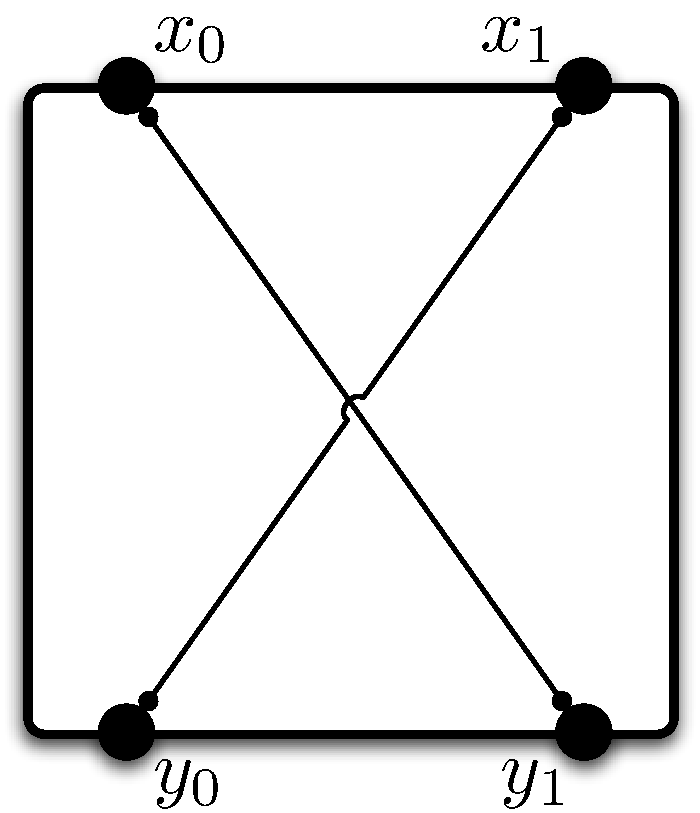
\includegraphics[viewport=0 0 390 360]{../../illustrations/BasicCrossingCircuit.pdf}}
    \caption{ Crossing process }
\end{figure}
\begin{eqnarray*}
   C(x_0,x_1,y_0,y_1,u) & \plogp   & x_1?(s).y_0!(s).(C(x_0,x_1,y_0,y_1,u)|u!) \nonumber \\
  & & + y_0?(s).x_1!(s).(C(x_0,x_1,y_0,y_1,u)|u!) \nonumber \\
  & & + x_0?(s).u?.y_1!(s).(C(x_0,x_1,y_0,y_1,u)) \nonumber \\
  & & + y_1?(s).u?.x_0!(s).(C(x_0,x_1,y_0,y_1,u)) \nonumber
\end{eqnarray*}

A crossing process has four ports $x_0,x_1,y_0,y_1$ and a hidden
synchronizer $u$. Each port has a partner port, linked as shown in the
diagram (note the relationship to Conway's $\pm 1$ tangles
\cite{Conway1970An-enumeration-}). For example, the first behavior (indicated by the first
term of the summand) is that the process listens at port $x_1$ for a
signal $s$ (which will come, if at all, via the wiring
process). Having heard $s$, the signal is passed directly to the port
$y_0$ where the signal is then broadcast via the wiring process. Then
the process alerts the hidden synchronizer $u$ that a signal has been
passed between the ports, while concurrently preparing itself for
further signal processing. The second summand represents a signal
passing along the same strand in the opposite direction. The third and
fourth summands are similar to the first two, except that before
passing any received signal to its partner port, the process waits for
a signal from the synchronizer $u$ before allowing the signal to
pass. So the role of $u$ is that of a traffic controller who gives
priority to traffic over the route between $x_1$ and $y_0$, mimicking
an over-crossing.

\subsection{Wirings}\label{sub:wirings} % (fold)

As an illustration of the expressive power of the formalism, taken
together with the short description of the process calculus in the next
section, the definitions below fully equip the interested reader to
verify that wire processes are lossless, infinite capacity buffers. 


\begin{eqnarray*}
    W(x,y) & \plogp & (\nu \; n \; m)(Waiting(x,n,m) | Waiting(y,m,n)) \nonumber \\
Waiting(x,c,n) & \plogp   & x?(v).(\nu \; m)(Cell(n,v,m) | Waiting(x,c,m)) \nonumber \\
  & & + c?(w).c?(c).Ready(x,c,n,w) \nonumber \\
  Ready(x,c,n,w) & \plogp  & x?(v).(\nu \; m)(Cell(n,v,m) | Ready(x,c,m,w)) \nonumber \\
  & & + x!(w).Waiting(x,c,n) \nonumber \\
  Cell(c,v,n) & \plogp & c!(v).c!(n).0 \nonumber
\end{eqnarray*}

The ports $x$ and $y$ in which $W$ is \emph{parameterized} may be
intuitively considered splice points in the knot diagram. We adopt
this terminology in the sequel.

One may well wonder why perfect buffers are chosen to represent
wires. For example, the following process intuitively captures a notion of wire.

\begin{equation*}
  Relay(x,y) := x?(s).y!(s).Relay(x,y) + y?(s).x!(s).Relay(x,y)
\end{equation*}

The problem is one of composition. Foreshadowing the method of proof,
in the sequel we will need to compose wires and crossings and have the
result act as a wire. For example, if $W(x,y)$ represents a candidate
for wire behavior, to model the first Reidemeister move we have a demand that

\begin{equation*}
  W(y_{0},y_{1}) \simeq (\nu \; x_{0} \; x_{1} \; w_{0} \; w_{1} )(W(y_{0},w_{0}) |(\nu \; u)C(x_{0},x_{1},w_{0},w_{1},u) | W(x_{0},x_{1}) | W(y_{1},w_{1}))
\end{equation*}

Again, the reader may verify that while this is true of buffers, it is
not true of the $Relay$ process defined above.
 

%\subsection{An example: the trefoil knot as a process}
The above intuitions are illustrated with an example, showing one way to
represent the trefoil knot as a process. Following the schema above,
the process encoding of the trefoil knot is a parallel composition of
three crossing circuits with a wiring harness whose design ensures that the
crossing circuits are connected to each other in a way that respects
the knot diagram. Additionally, we make each synchronization channel
local to each crossing via a restriction on that channel.

\begin{figure}[tbp]
\begin{center}
{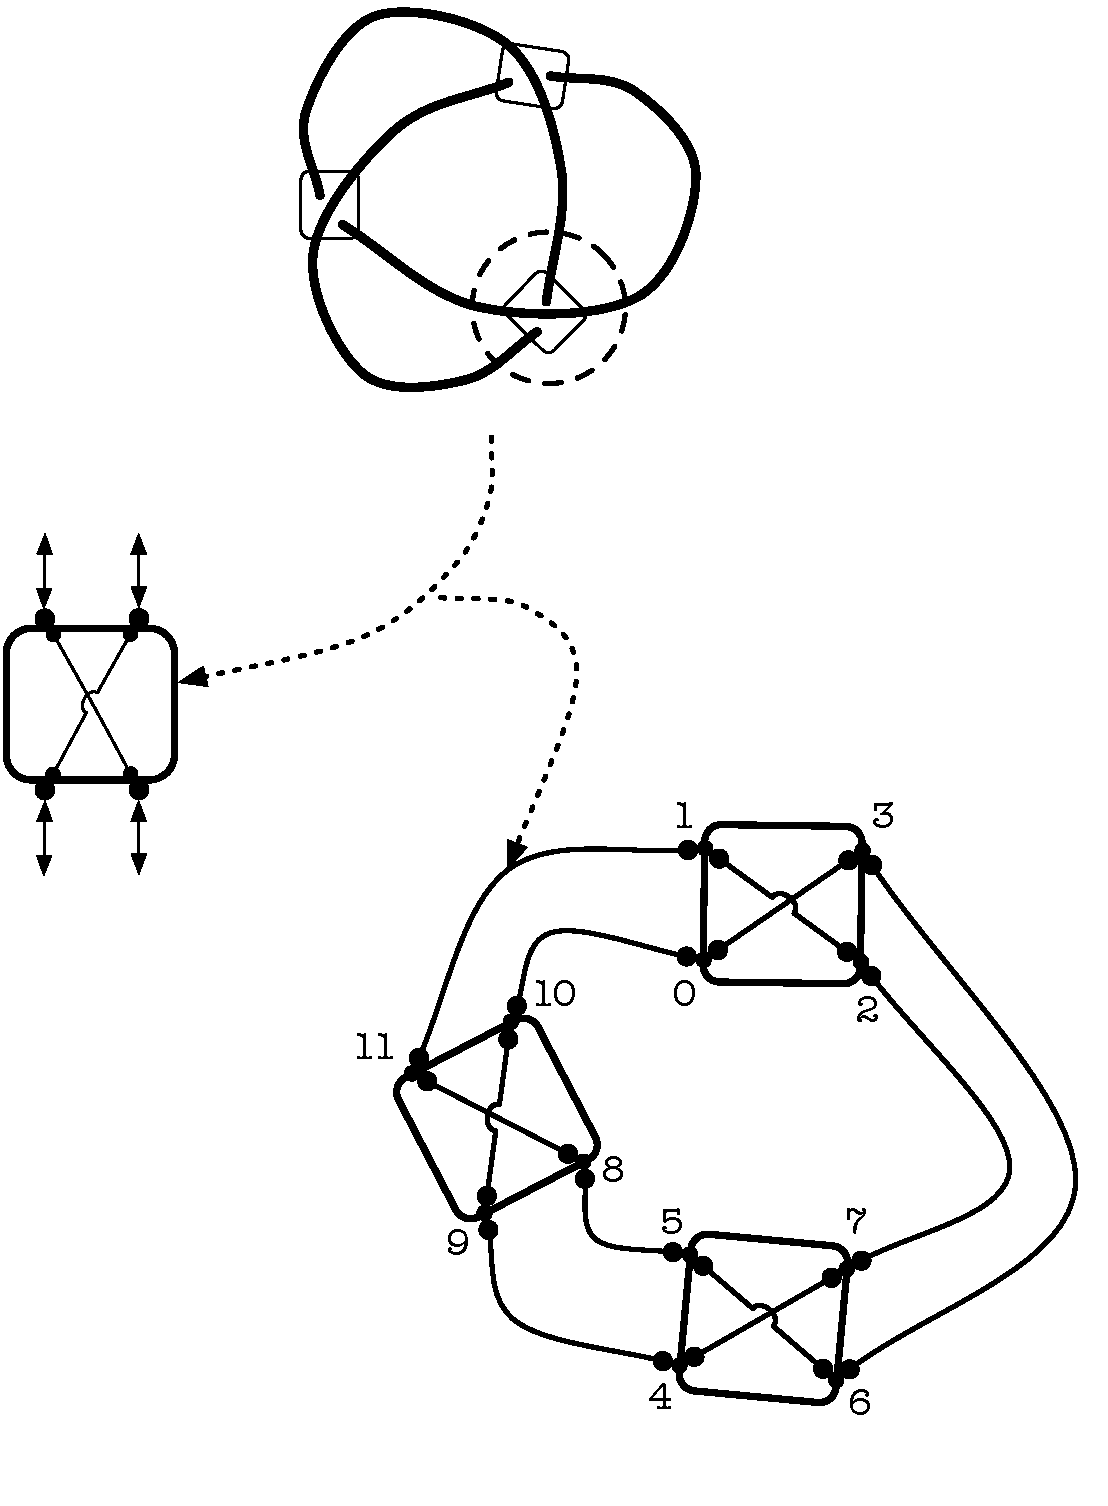
\includegraphics[width=3in]{../../illustrations/TrefoilMethodIllustration.pdf}}
\caption{ The $3_1$ (trefoil) knot as process. The ports in the
  circuit diagram have been labeled with the corresponding subscripted
  index in the process expression of the text.}
\end{center}
\end{figure}

% \begin{mathpar}
%   \meaningof{3_1} =
%    (v_0 ... v_{5}) (\nu \; u_0)C(v_0,v_1,v_2,v_3,u_0)
%     | W(v_2,v_7) | W(v_3,v_6)
%     \and \\
%     | (\nu \; u_1)C(v_4,v_5,v_6,v_7,u_1)
%     | W(v_4,v_9) | W(v_5,v_8)
%     \and \\
%     | (\nu \; u_2)C(v_8,v_9,v_{10},v_{11},u_2)
%     | W(v_{10},v_0) | W(v_{11},v_1)
% \end{mathpar}

\begin{align*}\label{eq:trefoil_encoding}
  \meaningof{3_1} = (v_0 ... v_{5}) & (\nu \; u_0) C(v_0,v_1,v_2,v_3,u_0) \\
   & | W(v_2,v_7) | W(v_3,v_6) \\
   & | (\nu \; u_1)C(v_4,v_5,v_6,v_7,u_1) \\
   & | W(v_4,v_9) | W(v_5,v_8) \\
   & | (\nu \; u_2)C(v_8,v_9,v_{10},v_{11},u_2) \\
   & | W(v_{10},v_0) | W(v_{11},v_1) 
\end{align*} 

%\subsection{The distinguishing power of dynamics}\label{sub:dynamic distinction} % (fold)

In summary, to each knot $\mathcal{K}$ the encoding associates an
invariant $\meaningof{K}$, an expression in a calculus of
message-passing processes via an encoding of a diagram of the
knot. More precisely, given the set of knot diagrams $\mathbb{K}$ and
the set of processes modulo structural equivalence $\mathbb {P}$ (see section
\ref{sub:the_syntax_and_semantics_of_the_notation_system}), the encoding induces a map, $\meaningof{-}: \mathbb{K} \to \mathbb
{P}$. Most importantly, the notion of equivalence of knots coincides perfectly with the notion of equivalence of
processes, i.e. bisimulation (written here and in the sequel
$\simeq$). Stated more formally,

\begin{theorem}[main]
\begin{eqnarray*}
    K_1 \sim K_2 & \iff & \meaningof{K_1} \simeq \meaningof{K_2}. \nonumber
\end{eqnarray*}
\end{theorem}

%Thus $\mathbb{K}$ may be taken to be the collection of isotopy classes of knots. 
In particular, in contrast to other invariants, the alignment of process
dynamics with knot characteristics is what enables the invariant
identified here to be perfectly distinguishing. As dicussed below,
among the other beneficial consequences of this alignment is the
ability to apply process logics, especially the spatial sub-family of
the Hennessy-Milner logics, to reason about knot characteristics and
knot classes.

We see moreover the possibility of a deeper connection. As mentioned
in the previous section, bisimulation has turned out to a powerful
proof technique in the theory of computation adaptable to a wide range
of situations and admitting a number of potent up-to techniques
\cite{DBLP:conf/lics/Sangiorgi04}. One of the central aims of this
research is to broaden the domain of applicability of
bisimulation-based proof methods.

% subsection basic_interpretation (end) 

% subsection basic_interpretation (end)

\subsection{The syntax and semantics of the notation system}\label{sub:the_syntax_and_semantics_of_the_notation_system} % (fold)

We now summarize a technical presentation of the calculus that
embodies our theory of dynamics. The typical presentation of such a
calculus follows the style of giving generators and relations on
them. The grammar, below, describing term constructors, freely
generates the set of processes, $\Proc$. This set is then quotiented
by a relation known as structural congruence and it is over this set
that the notion of dynamics is expressed. This presentation is
essentially that of \cite{MeredithR05} with the addition of
polyadicity and summation. For readability we have relegated some of
the technical subtleties to an appendix.

\subsubsection{Process grammar}\label{subsub:process_grammar}

\begin{mathpar}
  \inferrule* [lab=summation] {} {{M,N} \bc \pzero \;|\; x.A \;|\; M+N }
  \and
  \inferrule* [lab=agent] {} {{A} \bc (\vec{x})P \;| \; \clift{\vec{P}}}
  \and
  \inferrule* [lab=process] {} {{P,Q} \bc N \;| \;P|Q \;|\; \dropn{x}}
  \and
  \inferrule* [lab=name] {} {{x,y} \bc \quotep{P}}
\end{mathpar} 

Note that $\vec{x}$ (resp. $\vec{P}$) denotes a vector of names
(resp. processes) of length $|\vec{x}|$ (resp. $|\vec{P}|$). We adopt
the following useful abbreviations.

\begin{mathpar}
   x?(\vec{y}).P := x.(\vec{y})P \and  x\clift{\vec{P}} := x.\clift{\vec{P}}
   \and x!(y) := \lift{x}{\dropn{y}}
   \and \Pi_{i=0}^{n-1}P_i := P_0 | \ldots | P_{n-1}
\end{mathpar}

\subsubsection{Structural congruence}

\paragraph{Free and bound names and alpha-equivalence.} At the
core of structural equivalence is alpha-equivalence which identifies
process that are the same up to a change of variable. Formally, we
recognize the distinction between free and bound names. The free names
of a process, $\freenames{P}$, may be calculated recursively as
follows:

\begin{mathpar}
  \freenames{\pzero} := \emptyset
  \and \\
  \freenames{x?(\vec{y}).P} := \{ x \} \cup (\freenames{P} \setminus \{ \vec{y} \})
  \and 
  \freenames{x \clift{\vec{P}}} := \{ x \} \cup \{ \vec{P} \} 
  \and \\
  \freenames{P|Q} := \freenames{P} \cup \freenames{Q}
  \and
  \freenames{P + Q} := \freenames{P} \cup \freenames{Q}
  \and \\
  \freenames{\dropn{x}} := \{ x \}
\end{mathpar}

The bound names of a process, $\boundnames{P}$, are those names occurring in $P$
that are not free. For example, in $x?(y).0$, the name $x$ is free, while $y$ is bound.

\begin{definition}
Then two processes, $P,Q$, are alpha-equivalent if $P = Q\{\vec{y}/\vec{x}\}$ for
some $\vec{x} \in \boundnames{Q},\vec{y} \in \boundnames{P}$, where $Q\{\vec{y}/\vec{x}\}$
denotes the capture-avoiding substitution of $\vec{y}$ for $\vec{x}$ in $Q$.
\end{definition}

\begin{definition}
  The {\em structural congruence} \cite{SangiorgiWalker} , $\equiv$,
  between processes is the least congruence containing
  alpha-equivalence, satisfying the abelian monoid laws
  (associativity, commutativity and $\pzero$ as identity) for parallel
  composition $|$ and for summation $+$.
\end{definition}

\subsection{Name equivalence}

We take name equivalence, written $\nameeq$, to be the smallest
equivalence relation generated by the following rules.

\begin{mathpar}
\inferrule*[left=Quote-drop]
{ }
{ \quotep{\dropn{x}} \nameeq x }

\inferrule*[right=Struct-equiv]
{ P \scong Q }
{ \quotep{P} \nameeq \quotep{Q} }
\end{mathpar}

The astute reader will have noticed that the mutual recursion of names
and processes imposes a mutual recursion on alpha-equivalence and
structural equivalence via name-equivalence. Fortunately, all of this
works out pleasantly and we may calculate in the natural way, free of
concern. The reader interested in the details is referred to the
appendix \ref{appendix:rho_details}.

\subsection{Substitution}

We use $\Proc$ for the set of processes, $\QProc$ for the set of
names, and $\id{\{}\vec{y} / \vec{x} \id{\}}$ to denote partial maps,
$s : \QProc \rightarrow \QProc$. A map, $s$ lifts, uniquely, to a map
on process terms, $\widehat{s} : \Proc \rightarrow \Proc$ by the
following equations.

\begin{mathpar}
  (0) \psubstp{Q}{P} := 0 \\
  (R \juxtap S) \psubstp{Q}{P}
  :=    
  (R)\psubstp{Q}{P} \juxtap (S) \psubstp{Q}{P} \\
  (x?(y).R) \psubstp{Q}{P}    
  :=    
  (x)\substp{Q}{P} (z)\concat( (R \psubstn{z}{y}) \psubstp{Q}{P} ) \\
  (\lift{x}{R}) \psubstp{Q}{P}  
  :=
  \lift{(x)\substp{Q}{P}}{ R \psubstp{Q}{P} } \\
%   (\dropn{x})  \psubstp{Q}{P}       
%   := 
%   \left\{ 
%     \begin{array}{ccc} 
%       \dropn{\quotep{Q}} & & x \nameeq \quotep{P} \\
%       \dropn{x} & & otherwise \\
%     \end{array}
%   \right. 
  (\dropn{x})  \psubstp{Q}{P}       
  := 
  \left\{ 
    \begin{array}{ccc} 
      Q & & x \nameeq \quotep{P} \\
      \dropn{x} & & otherwise \\
    \end{array}
  \right.
\end{mathpar}
 

where

\begin{eqnarray}
  (x)\id{\{} \lpquote Q \rpquote / \lpquote P \rpquote \id{\}}            = 
  \left\{ 
    \begin{array}{ccc}
      \lpquote Q \rpquote & & x \nameeq \lpquote P \rpquote \\
      x & & otherwise \\
    \end{array}
  \right. \nonumber
\end{eqnarray}

and $z$ is chosen distinct from $\quotep{P}$, $\quotep{Q}$, the free
names in $Q$, and all the names in $R$. Our $\alpha$-equivalence will
be built in the standard way from this substitution.

\begin{remark}\label{rem:no_self_referential_names}
  One consequence of these definitions is that $\forall P. \quotep{P}
  \not\in \freenames{P}$.
\end{remark}

\subsection{ Dynamic quote: an example }

Anticipating something of what's to come, consider applying the
substitution, $\widehat{\id{\{}u / z \id{\}}}$, to the following pair
of processes, $\lift{w}{y!(z)}$ and $w[ \lpquote y!(z) \rpquote ]$.

\begin{eqnarray}
	\lift{w}{y!(z)}\widehat{\id{\{}u / z \id{\}}}
		& = &
		\lift{w}{y!(u)} \nonumber\\
	w[ \lpquote y!(z) \rpquote ] \widehat{ \id{\{}u / z \id{\}} }
		& = &
		w[ \lpquote y!(z) \rpquote ] \nonumber
\end{eqnarray}

Because the body of the process between quotes is impervious to
substitution, we get radically different answers. In fact, by
examining the first process in an input context,
e.g. $x?(z).\lift{w}{y!(z)}$, we see that the process under the lift
operator may be shaped by prefixed inputs binding a name inside it. In
this sense, the lift operator will be seen as a way to dynamically
construct processes before reifying them as names.

Finally equipped with these standard features we can present the
dynamics of the calculus.

\subsubsection{Operational semantics} 

Finally, we introduce the computational dynamics. What marks these
algebras as distinct from other more traditionally studied algebraic
structures, e.g. vector spaces or polynomial rings, is the manner in
which dynamics is captured. In traditional structures, dynamics is typically
expressed through morphisms between such structures, as in linear maps
between vector spaces or morphisms between rings. In algebras
associated with the semantics of computation, the dynamics is
expressed as part of the algebraic structure itself, through a
reduction reduction relation typically denoted by $\red$. Below, we
give a recursive presentation of this relation for the calculus used
in the encoding.

\begin{mathpar}
  \inferrule* [lab=Comm] { x_{src} \nameeq x_{trgt} \\ \vec{y} \cap \vec{v} = \emptyset \\ |\vec{y}| = |\vec{z}|} { R_{L} + x_{trgt}?(\vec{y})P \; | \; x_{src}\clift{\vec{Q}} + R_{R} \red P\{\vec{\quotep{Q}}/\vec{y}\} }
  \and \\
  \inferrule* [lab=Par] {{P} \red {P}'} {{{P} | {Q}} \red {{P}' | {Q}}}
  \and
  \inferrule* [lab=Equiv]{{{P} \scong {P}'} \andalso {{P}' \red {Q}'} \andalso {{Q}' \scong {Q}}}{{P} \red {Q}}
\end{mathpar}

%We write $\wred$ for $\red^*$, and $P\red$ if $\exists Q $ such that $ P \red Q$.
We write $P\red$ if $\exists Q $ such that $ P \red Q$ and $P\not\red$, otherwise.

\section{Replication}

As mentioned before, it is known that replication (and hence
recursion) can be implemented in a higher-order process algebra
\cite{SangiorgiWalker}. As our first example of calculation with the
machinery thus far presented we give the construction explicitly in
the {\rhoc}.

\begin{eqnarray}
	D_{x} & := & \prefix{x}{y}{(\binpar{\outputp{x}{y}}{\dropn{y}})} \nonumber\\
	\bangp_{x}{P} & := & \binpar{\lift{x}{\binpar{D_{x}}{P}}}{D_{x}} \nonumber
\end{eqnarray}

\begin{eqnarray}
	\bangp_{x}{P} & & \nonumber\\
	=
	& \lift{x}{(\prefix{x}{y}{(\outputp{x}{y} | \dropn{y})) | P}} 
	      | \prefix{x}{y}{(\outputp{x}{y} | \dropn{y})} & \nonumber\\
	\red
	& (\outputp{x}{y} | \dropn{y})\substn{\quotep{(\prefix{x}{y}{(\dropn{y} | \outputp{x}{y})) | P}}}{y} & \nonumber\\
	=
	& \outputp{x}{\quotep{(\prefix{x}{y}{(\outputp{x}{y} | \dropn{y})) | P}}}
	  | {(\prefix{x}{y}{(\outputp{x}{y} | \dropn{y})) | P}} & \nonumber\\
	\red
	& \ldots & \nonumber\\
	\red^*
	& P | P | \ldots & \nonumber
\end{eqnarray}

Of course, this encoding, as an implementation, runs away, unfolding
$\bangp{P}$ eagerly. A lazier and more implementable replication
operator, restricted to input-guarded processes, may be obtained as follows.

\begin{eqnarray}
\bangp{\prefix{u}{v}{P}} 
	:= 
	\binpar{\lift{x}{\prefix{u}{v}{(\binpar{D(x)}{P})}}}{D(x)} \nonumber
\end{eqnarray}

\begin{remark}
  Note that the lazier definition still does not deal with summation
  or mixed summation (i.e. sums over input and output). The reader is
  invited to construct definitions of replication that deal with these
  features. 

  Further, the definitions are parameterized in a name, $x$. Can you,
  gentle reader, make a definition that eliminates this parameter and
  guarantees no accidental interaction between the replication
  machinery and the process being replicated -- i.e. no accidental
  sharing of names used by the process to get its work done and the
  name(s) used by the replication to effect copying. This latter
  revision of the definition of replication is crucial to obtaining
  the expected identity $!!P \sim !P$.
\end{remark}

\begin{remark}\label{rem:paradoxical_combinator}
  The reader familiar with the lambda calculus will have noticed the
  similarity between $D$ and the paradoxical combinator.

  [Ed. note: the existence of this seems to suggest we have to be more
  restrictive on the set of processes and names we admit if we are to
  support no-cloning.]
\end{remark}

\subsubsection{Bisimulation}

The computational dynamics gives rise to another kind of equivalence,
the equivalence of computational behavior. As previously mentioned
this is typically captured \emph{via} some form of bisimulation.

% The notion we use in this paper is weak barbed bisimulation
% \cite{milner91polyadicpi}.

The notion we use in this paper is derived from weak barbed
bisimulation \cite{milner91polyadicpi}. 

\begin{definition}
An \emph{observation relation}, $\downarrow_{\mathcal N}$, over a set
of names, $\mathcal N$, is the smallest relation satisfying the rules
below.

\infrule[Out-barb]{y \in {\mathcal N}, \; x \nameeq y}
		  {\outputp{x}{v} \downarrow_{\mathcal N} x}
\infrule[Par-barb]{\mbox{$P\downarrow_{\mathcal N} x$ or $Q\downarrow_{\mathcal N} x$}}
		  {\binpar{P}{Q} \downarrow_{\mathcal N} x}

We write $P \Downarrow_{\mathcal N} x$ if there is $Q$ such that 
$P \wred Q$ and $Q \downarrow_{\mathcal N} x$.
\end{definition}

\begin{definition}
%\label{def.bbisim}
An  ${\mathcal N}$-\emph{barbed bisimulation} over a set of names, ${\mathcal N}$, is a symmetric binary relation 
${\mathcal S}_{\mathcal N}$ between agents such that $P\rel{S}_{\mathcal N}Q$ implies:
\begin{enumerate}
\item If $P \red P'$ then $Q \wred Q'$ and $P'\rel{S}_{\mathcal N} Q'$.
\item If $P\downarrow_{\mathcal N} x$, then $Q\Downarrow_{\mathcal N} x$.
\end{enumerate}
$P$ is ${\mathcal N}$-barbed bisimilar to $Q$, written
$P \wbbisim_{\mathcal N} Q$, if $P \rel{S}_{\mathcal N} Q$ for some ${\mathcal N}$-barbed bisimulation ${\mathcal S}_{\mathcal N}$.
\end{definition}

\subsubsection{Contexts}

One of the principle advantages of computational calculi like the
$\pi$-calculus is a well-defined notion of context,
contextual-equivalence and a correlation between
contextual-equivalence and notions of bisimulation. The notion of
context allows the decomposition of a process into (sub-)process and
its syntactic environment, its context. Thus, a context may be
thought of as a process with a ``hole'' (written $\Box$) in it. The
application of a context $M$ to a process $P$, written $M[P]$, is
tantamount to filling the hole in $M$ with $P$. In this paper we do
not need the full weight of this theory, but do make use of the notion
of context in the proof the main theorem. 

\begin{mathpar}
  \inferrule* [lab=summation] {} {{M_{M},M_{N}} \bc \Box \;|\; x.M_{A} \;|\; M_{M}+M_{N}}
  \and
  \inferrule* [lab=agent] {} {{M_{A}} \bc (\vec{x})M_{P} \;| \; \clift{P_0,\ldots,M_{P},\ldots,P_N}}
  \and \\
  \inferrule* [lab=process] {} {{M_{P}} \bc M_{N} \;| \;P|M_{P} }
\end{mathpar} 

\begin{definition}[contextual application] Given a context $M$, and
  process $P$, we define the \emph{contextual application}, $M[P] :=
  M\{P/\Box\}$. That is, the contextual application of M to P is the
  substitution of $P$ for $\Box$ in $M$.
\end{definition}

\subsubsection{Contextual duality}

Note that contexts extend the quotation operation to a family of
operations from processes to names. Given a context, $M$, we can
define a new map, $\quotep{M}$ by $\quotep{M}[P] := \quotep{M[P]}$. To
foreshadow what is to come we observe that these operations enjoy a
duality with processes very much like the duality between vectors and
maps from vectors to scalars.

Further, because the calculus is essentially higher-order, we have a
correspondence between contexts and processes. More specifically,
given a name $x$ and a context $M$ we can construct $M^{*}_{x}$ such
that 

\begin{mathpar}
  M^{*}_{x} | \lift{x}{P} \red M[P]
\end{mathpar}

namely,

\begin{mathpar}
  M^{*}_{x} := x?(u).M[\dropn{u}]
\end{mathpar}

\subsection{Additional notation}

It will sometimes be convenient to denote the process a name
quotes. We already have the notation $x = \quotep{P}$, but it will be
convenient to introduce an alternate notation, $\procn{x}$, when we
want to emphasize the connection to the use of the name. Note that, by
virtue of name equivalence, $\quotep{\procn{x}} \nameeq x$; so, the
notation is consistent with previous definitions.

Also, we will avail ourselves of the notation $x^{L}$ and $x^{R}$ to
denote injections of a name into disjoint copies of the name
space. There are numerous ways to accomplish this. One example can be
found in \cite{MeredithR05}. This notation overloads to vectors of
names: $\vec{x}^{\pi} := (x_{i}^{\pi} \; | \; 0 \leq i < |\vec{x}| )$ where $\pi \in \{L,R\}$.

We also use $P^{\Box} := P|\Box$.

% subsection the_syntax_and_semantics_of_the_notation_system (end)    

\section{Interpretation of QM}
\subsection{Supporting definitions}

To provide our interpretation of quantum mechanics we need to develop
a number of supporting definitions. As the reader familiar with
process algebraic systems can readily verify, these definitions make
\emph{essential} use of the reflective operations and as such identify
this calculus as uniquely suited to this particular task.

Among these operations we find a notion of \emph{multiplication} of
names that interacts well with a notion of \emph{tensor product} of
processes. Even more intriguingly, we find a notion of a \emph{dual}
to a process in the form of maps from processes to names. While
notions of composite names have been investigated in the process
algebraic literature, it is the fact that names reflect process
structure that enables the collection of duals to enjoy an algebraic
structure dual to the collection of processes (i.e. there are
operations available to duals that reflect the operations on
processes). Moreover, it is this structure that enables an effective
definition of inner product.

\subsubsection{Multiplication}
\begin{mathpar}
  \quotep{Q} \cdot \quotep{R} := \quotep{Q|R}
  \and \\
  \quotep{Q} \cdot P := P\{ \quotep{Q|R} / \quotep{R} : \quotep{R} \in \freenames{P} \}
\end{mathpar}

\paragraph{Discussion}
The first equation needs little explanation; the second says that each
free name of the process is replaced with the multiplication of that
name by the scalar. Multiplication of a scalar (name) by a state
(process) results in a process all the names of which have been `moved
over' by parallel composition with the process the scalar
quotes. There is a subtlety that the bound names have to be
manipulated so that multiplied names aren't accidentally
captured. There are many ways to achieve this.

\begin{remark}\label{rem:multiplication_identities}
  The reader is invited to verify that for all $x,y,z \in \QProc$ and $P \in \Proc$
  \begin{mathpar}
    x \cdot \quotep{0} \equiv x 
    \and
    x \cdot y \equiv y \cdot x
    \and
    x \cdot (y \cdot z) \equiv (x \cdot y) \cdot z
    \and \\
    \quotep{0} \cdot P \equiv P
    \and \\
    x \cdot (y \cdot P) \equiv (x \cdot y) \cdot P
    \and \\
    x \cdot (P|Q) \equiv (x \cdot P) | (x \cdot Q)
    \and \\    
  \end{mathpar}
\end{remark}

\subsubsection{Tensor product}

We define a tensor product on processes by structural induction.

\paragraph{Tensor of sums} First note that all summations, including
$\pzero$ and sequence, can be written $\Sigma_{i} x_{i}.A_{i} +
\Sigma_{j} x_{j}.C_{j}$, where we have grouped input-guarded processes
together and output-guarded processes together.

Thus, we can define the tensor product of two summations, $N_{1}\otimes N_{2}$, where

\begin{mathpar}
  N_{1} := \Sigma_{i} x_{i}.A_{i} + \Sigma_{j} x_{j}.C_{j}
  \and
  N_{2} := \Sigma_{i'} y_{i'}.B_{i'} + \Sigma_{j'} y_{j'}.D_{j'} 
\end{mathpar}

as follows.

\begin{mathpar}
  \Sigma_{i} x_{i}.A_{i} + \Sigma_{j} x_{j}.C_{j} \otimes \Sigma_{i'}
  y_{i'}.B_{i'} + \Sigma_{j'} y_{j'}.D_{j'} 
  \and \\
  := \; \Sigma_{i} \Sigma_{i'} \quotep{\stackrel{\vee}{x_{i}}| \stackrel{\vee}{y_{i'}}}.(A_{i}\otimes B_{i'}) \; | \; \Sigma_{i'} \Sigma_{i} \quotep{\stackrel{\vee}{y_{i'}}|\stackrel{\vee}{x_{i}}}.(B_{i'}\otimes A_{i})
  \and
  \;\; | \;\; \Sigma_{j} \Sigma_{j'} \quotep{\stackrel{\vee}{x_{j}}|\stackrel{\vee}{y_{j'}}}.(A_{j}\otimes B_{j'}) \; | \; \Sigma_{j'} \Sigma_{j} \quotep{\stackrel{\vee}{y_{j'}}|\stackrel{\vee}{x_{j}}}.(B_{j'}\otimes A_{j})
\end{mathpar}

\begin{remark}
  Do we need to $x^{L}$ and $y^{R}$ for this construction as well?
\end{remark}

\paragraph{Tensor of parallel compositions} Next, we distribute tensor
over par.

\begin{mathpar}
  P_{1}|P_{2} \otimes Q_{1}|Q_{2} := (P_{1} \otimes Q_{1}) | (P_{1}
  \otimes Q_{2}) | (P_{2} \otimes Q_{1}) | (P_{2} \otimes Q_{2})
\end{mathpar}

\paragraph{Tensor with dropped names} We treat tensor of a
process with a dropped name as parallel composition.

\begin{mathpar}
  P \otimes \dropn{x} := P | \dropn{x}
\end{mathpar}

\paragraph{Tensor of agents}

Finally, we need to define tensor on agents. Note that the definition
of tensor on summations only tensors inputs with inputs and outputs
with outputs. Thus, we only have to define the operation on
``homogeneous'' pairings.

\begin{mathpar}
  (\vec{x})P \otimes (\vec{y})Q
  \and \\
  := (x_{0}^{L}|y_{0}^{R},\ldots,x_{0}^{L}|y_{n}^{R},\ldots,x_{m}^{L}|y_{0}^{R},\ldots,x_{m}^{L}|y_{n}^R)(P\{ \vec{x}^{L}/\vec{x}\} \otimes Q \{ \vec{y}^{R}/\vec{y}\})
  \and \\
  \clift{\vec{P}} \otimes \clift{\vec{Q}}
  \and \\
  := \clift{P_{0}\otimes Q_{0},\ldots,P_{0}\otimes Q_{n},\ldots,P_{m}\otimes Q_{0},\ldots,P_{m}\otimes Q_{n}}
\end{mathpar}

\begin{remark}
  Observe that arities of tensored abstractions matches arities of
  tensored concretions if the original arities matched. Note also that
  the length of the arities corresponds to the increase in dimension
  we see in ordinary vector space tensor product.
\end{remark}

\begin{remark}
  Operationally, this definition distributes the tensor down to
  components ``linked'' by summation. Tensor over summation is
  intriguing in that it mixes names. Moreover, as a consequence of the
  way it mixes names we have the identities for all $x \in \QProc$ and
  $P,Q \in \Proc$

  \begin{mathpar}
    (x \cdot P) \otimes Q \equiv x \cdot (P \otimes Q) \equiv P \otimes (x \cdot Q)
    \and \\
    P \otimes \pzero \equiv P
  \end{mathpar}

  that the reader is invited to verify.
\end{remark}

\subsubsection{Annihilation}
\begin{mathpar}
  P^{\perp} := \{ Q : \forall R. P|Q \red^{*} R \Rightarrow R \red^{*} \pzero \}
  \and \\
  \annihilate{P} := \Sigma_{Q \in P^{\perp}} \quotep{Q}?(y).(\dropn{y}|Q) | \Sigma_{Q \in P^{\perp}} \quotep{Q}\clift{\Box}
\end{mathpar}

\paragraph{Discussion} The reader will note that $P^{\perp}$ is a
\emph{set} of processes, while $\annihilate{P}$ is a
\emph{context}. We call the set $P^{\perp}$ the \emph{annihilators} of
$P$. The parallel composition of a process in the annihilators of $P$
with $P$ will result in a process, the state space of which has all
paths eventually leading to $\pzero$. Execution may endure loops; but
under reasonable conditions of fairness (naturally guaranteed under
most notions of bisimulation) such a composite process cannot get
stuck in such a loop and will, eventually pop out and terminate.

The context $\annihilate{P}$ is ready and willing to ``take the
$P$ out of'' the process to which it is applied. It will effectively
transmit the code of the process to which it is applied to one of the
annihilators and run the process against it.

\begin{remark}
  Note that ${\annihilate{P}}^*$ is the abstraction corresponding to
  context $\annihilate{P}$. We will set $\dualize{P} := {\annihilate{P}}^*$.
\end{remark}

\subsubsection{Evaluation}
We fix $M$ a domain of fully abstract interpretation with an equality
coincident with bisimulation. We take $\meaningof{\cdot} : \Proc \to
M$ to be the map interpreting processes and $\nmeaningof{\cdot} : \M
\to Proc$ to be the map running the other way. Then we define

\begin{mathpar}
  \int P := \nmeaningof{\meaningof{P}}
\end{mathpar}

\paragraph{Discussion}
There are many fully abstract interpretations of Milner's
$\pi$-calculus. Any of them can be used as a basis for interpreting
the reflective calculus here. Equipped with such a domain it is
largely a matter of grinding through to check that the Yoneda
construction for the normalization-by-evaluation program can be
extended to this setting.

\begin{remark}
  The reader is invited to verify that $\int (\annihilate{P}[P]) = 0$,
  and equivalently $(\nu\; x)\int \dualize{P}\langle x \rangle |
  x\clift{P} = 0$.
\end{remark}

\subsection{Quantum mechanics}

\subsubsection{What is the quantum mechanical notion of continuation?}\label{sec:quantum_continuation}

Imagine the following experimental set-up. Alice, our intrepid quantum
investigator, prepares a state by performing some operation on some
initial state. Then she performs some measurement to obtain an
observation. Using the information of the observation, she selects a
new initial state, operation and measurement and repeats the steps
above. She iterates this procedure until she obtains some desired
observation. What is the expression of this procedure in the language
of quantum mechanics?

\begin{figure}[htp]\label{fig:iterated_experiment}
%  \fbox{
    \begin{lstlisting}[mathescape]
      $\mathcal{E} ::=$
      let S = $U \state{L}$ in (* prepare state*)
      let m = $\innerprod{M}{S}^2$ in (* take measurement *)
      match m with (* use m to decide next experiment *)
      v$_0$ -> $\mathcal{E}$
      | $\ldots$
      | v$_N$ -> $\mathcal{E}$
      | v$_{Exit}$ -> m (* return observation *)
    \end{lstlisting}
%    }
  \caption{Iterated experiment schematic}
\end{figure}

Figure \ref{fig:iterated_experiment} gives a schematic description of
such an iterated experimental procedure. The question is how do we
write down this iterated procedure without stepping outside the
language of quantum mechanics? Note that accounts of famous composite
quantum experiments, like the Stern-Gerlach experiment leave the
language of quantum mechanics to describe the iterated experiment.

We ask this question for many reasons, but one of them is to help set
up the exegesis of our interpretation. In our framework
\emph{everything} is a computation, both the quantum operations and
processes (classical or quantum) that invoke those operations. There
is no need to step out of the conceptual (and more pragmatically, the
computational) framework to describe these kinds of experiments. More
to the point, the framework we are proposing is -- like the hybrid
functional language employed in the schema -- \emph{compositional}:
experiments, computations are built out of experiments and
computations. This is of enormous pragmatic value if we are to build
and reason about systems of significant scale.

\begin{remark}
  It is also worth noting in this connection that this schema is the
  core of a wide range of recursive functions. Further, this
  connection to calculations of fixpoints makes it a close neighbor of
  search techniques like natural selection and the scientific
  method. This is a theme to which we will return, for quantum
  information seems very \emph{unlife-like} in it's uncloneable,
  undeleteable nature.
\end{remark}

Returning the matter of the computational interpretation, our
interpretation will take the form of a map, written
$\meaningof{-}(-)$, from expressions in Dirac notation to expressions
in our target reflective calculus. The map takes an \emph{ancillary}
argument, a channel along which to communicate results to subsequent
computations. This is how we communicate, for example, the results of
taking a measurement to a subsequent step in an experiment.

\subsubsection{Interpretation}

Table \ref{tbl:core_qm_op_defns} gives the core operational
correspondences. It is meant as an intuitive guide.

\begin{table}[htp]\label{tbl:core_qm_op_defns}
  \center{
    \fbox{
      \begin{tabular}{c|c}
        quantum mechanics & process calculus \\
        \hline
        scalar & $x := \quotep{P}$ \\
        state vector & $\state{P} := P$ \\
        dual & $\state{P}^{*} := \event{\annihilate{P}} := \quotep{\annihilate{P}}[-]$ \\
        matrix & $ \Sigma_{\alpha} \state{P_{\alpha}}x_{\alpha}\event{Q_{\alpha}}$ \\
        vector addition & $\state{P} + \state{Q} := \state{P | Q}$ \\
        tensor product & $\state{P} \otimes \state{Q} := \state{P \otimes Q}$ \\
        inner product & $\innerprod{P}{Q} := \quotep{\int \annihilate{P}[Q]}$ \\
      \end{tabular}
    }
  }
  \caption{QM - operational definitions}
\end{table}

\paragraph{Discussion}
The process algebraic view of a state is called, ironically, a
process, and that is what we map vectors to in our interpretation. It
has long been noted in the process algebraic community that names play
a role somewhat similar to scalars in a vector space. What is unique
about the reflective calculus, and makes it suitable for an
interpretation of this form is that with the structure of names
reflecting the structure of processes we can both make this similarity
in a precision instrument; and find a notion of \emph{dual} to a
state. 

If we posit names as scalars, then in perfect analogy with vector
spaces a dual is a map from processes to names. We actually have two
candidates for this interpretation: nominal contexts, $\quotep{M}$,
and their corresponding abstraction, $\quotep{M}^{*}$. The goal of
supporting a notion of continuation selects the latter of the two for
our interpretation.

Taking these as the basis of the interpretation together with the
algebraic identities required by the Dirac notation more or less fixes
the definitions of the rest of the operations. Among the interesting
particularities, the definition of inner product finds near perfect
mirroring of the Feyman interpretation.

\begin{mathpar}
  \inferrule* [lab=states] {} {\meaningof{\state{P}}(c) = c?(l,r).r\clift{P}}
  \and
  \inferrule* [lab=events] {} {\meaningof{\event{P}}(c) = (x)c?(l,r).l\clift{\dualize{P}\langle x \rangle} } 
  \and
  \inferrule* [lab=vector addition] {} {\meaningof{\state{P} + \state{Q}}(c) = \meaningof{\state{P | Q}}(c)}
  \and
  \inferrule* [lab=tensor product] {} {\meaningof{\state{P} \otimes \state{Q}}(c) = \meaningof{\state{P\otimes Q}}(c)}
  \and
  \inferrule* [lab=inner product] {} {\meaningof{\innerprod{P}{Q}}(c) = (\nu\; x)c\clift{\int \dualize{P}\langle x \rangle | x\clift{Q}}}
  \and
  \inferrule* [lab=matrix] {} {\meaningof{\fprmatrix{P}{x}{Q}}(c) = \\\\ (u)(\nu \; lr) c!(l,r).(l?(e). (\nu\; y)\meaningof{\innerprod{\dropn{e}}{Q}}(x) | x?(z).x?(a).c\clift{(\dualize{P}\sigma(z,a))\langle u \rangle}|y!(x) \\\\
    + r?(e). (\nu\; x)\meaningof{\innerprod{P}{\dropn{e}}}(x) | x?(z).x?(a).c\clift{Q\sigma(z,a)}|x!(x_{\alpha}))}  
  \and
  \inferrule* [lab=matrix application] {} {\meaningof{(\fprmatrix{P}{x}{Q})(\state{S})}(c) = (\nu\; c'u)\meaningof{\fprmatrix{P}{x}{Q}}(c')\langle u \rangle | \meaningof{\state{S}}(c') | c'?(a).c!(a)
  \\\\
  \meaningof{(\fprmatrix{P}{x}{Q})(\event{S})}(c) = (\nu\; c'u)\meaningof{\fprmatrix{P}{x}{Q}}(c')\langle u \rangle | \meaningof{\event{S}}(c') | c'?(a).c!(a)}
\end{mathpar}

where

\begin{mathpar}
  P\sigma(z,a) := P\{ z\cdot a\cdot r/r : r \in \freenames{P} \}
\end{mathpar}

\begin{remark}
  The reader is invited to verify that
  \begin{mathpar}
    \meaningof{\innerprod{P}{Q}}(c)
    \and \\
    \wbbisim 
    \and \\
    %\and
    (\nu\; x)(\nu c'lr)\meaningof{\event{P}}(c')\langle x \rangle \;|\; \meaningof{\state{Q}}(c')
    %\and
    |\; c'!(l,r).l?(p).r?(q).c\clift{\int \dropn{p} | x!(q)}
  \end{mathpar}
  This provides a (more) compositional definition of inner product. It
  also illustrates an important point of the computational
  interpretation. We have a notion of equivalence providing a crucial
  proof method: bisimulation.
\end{remark}

\begin{remark}
  Assuming $\int (\annihilate{P}[P]) = 0$, the reader is
  invited to verify that $(\fprmatrix{P}{x}{P})(\state{P}) = x \cdot \state{P}$.
\end{remark}

% \begin{remark}
%   The reader is invited to verify that $\innerprod{P}{Q}$ could
%   equally well have been written $\quotep{\int \stackrel{\vee}{x}}$
%   where $x = \event{\annihilate{P}}(Q)$.

%   One of the motivations for this remark is that there is another way
%   to factor these operations. We could package up evaluation in the dual:

%   \begin{mathpar}
%     \state{P}^{*} := \event{\int \annihilate{P}} := \quotep{\int \annihilate{P}}[-]
%   \end{mathpar}

%   and then have inner product defined by
  
%   \begin{mathpar}
%     \innerprod{M}{Q} := \event{M}(Q)
%   \end{mathpar}

%   where we use $M$ to label the dual to emphasize that it is a context.

%   Hopefully, experience with the calculations will provide guidance on
%   the best factoring.
% \end{remark}

\begin{remark}\label{rem:abstract_scalars}
  Assuming $\int (\annihilate{P}[P]) = 0$, the reader is
  invited to verify that $\forall P,Q. (\prmatrix{0}{Q})(\state{0}) =
  \state{0}$ and dually $(\prmatrix{P}{0})(\event{0}) = \event{0}$.
\end{remark}

\subsubsection{Interpreting continuations}

As promised, we can combine these interpretations with standard
semantics for conditionals and continuations to provide an
interpretation of the iterated experiment.

\begin{lstlisting}[mathescape]      
  $\ldb$ let S = $U \state{L}$ in 
  let m = $\innerprod{M}{S}^2$ in 
  match m with 
  v$_0$ -> $\mathcal{E}$
  | $\ldots$
  | v$_N$ -> $\mathcal{E}$
  | v$_{Exit}$ -> m $\rdb(c)$
  $=$
  $(\nu\; c')\meaningof{\innerprod{M}{U\state{L}}}(c')$
  $| c'?(m).m!(m) | \Sigma_{i=0}^{N}v_{i}?(m).\meaningof{\mathcal{E}} + v_{Exit}?(m).c!(m)$
\end{lstlisting}

\paragraph{A quick tally}
Already the interpretation is beginning to show signs of
promise. First of all, it is no more notationally cumbersome than the
notation used in QM calculations. Beyond syntax, we have a new proof
principle in hand and the ability to reason about more complex
experimental situations than is directly calculable in ordinary
quantum mechanics.

\subsubsection{Adjointness}

We need to give a definition of $(\cdot)^{\dagger}$ for matrices. The
obvious candidate definition is
\begin{mathpar}
\meaningof{(\fprmatrix{P}{x}{Q})^{\dagger}}(c)
= (\nu\; u)\meaningof{\fprmatrix{\dualize{Q}\langle u \rangle}{\overline{x}}{\dualize{P}\langle u \rangle}}(c) 
\end{mathpar}

% But, $(Q_{\alpha}^{\underline{\perp}})^{*}$ requires a name along
% which to communicate the process to achieve the context application.

\begin{remark}
  i'm a little worried that i don't (yet) have proper support for
  complex conjugacy. But, the observation above may give us a
  clue. According to Abramsky, it must be the case that the scalars
  are iso to the homset of the identity for the tensor -- which the
  observation above (\ref{rem:abstract_scalars}) characterizes. For
  now, we will simply bookmark the notion with $\overline{x}$.
\end{remark}

\subsubsection{Basis for a basis}
If processes label states and ``addition'' of states (a.k.a. vector
addition) is interpreted as parallel composition, what corresponds to
notions of linear independence and basis? Here, we recall that Yoshida
has developed a set of \emph{combinators} for an asynchronous verison
of Milner's $\pi$-calculus \cite{DBLP:conf/concur/Yoshida98}. These
are a finite set of processes such any process can be expressed as
parallel composition of these combinators together with liberal uses
of the new operator and replication. We can simply give a translation
of these into the present calculus and have reasonable expectation
that the property carries over. That is, that the resultant set allows
to express all processes via parallel composition. Note, however, that
there is no new operator or replication in this calculus. As a result,
we expect that the corresponding set is actually infinite. That is, we
expect that the space is actually infinite dimensional.

\begin{remark}
  The reader familiar with the lambda calculus may reasonably object:
  certainly, the collection $S$, $K$ and $I$ is a finite set of
  combinators \cite{Barendregt84}. Shouldn't we expect to see a finite
  set of combinators for an effectively equivalent system? i am very
  sympathetic to this critique and feel it warrants full attention. On
  the other hand, i also have in mind the following analogy. The
  natural numbers, as a monoid under addition, has exactly $1$
  generator, while the natural numbers, as a monoid under
  multiplication, has countably many generators (the primes). We
  observe that the application of the lambda calculus is much less
  resource sensitive than the parallel composition of the
  $\pi$-calculus. Could it be the case that we have an analogy of the
  form
  
  \begin{mathpar}
    m + n : MN :: m*n : M|N
  \end{mathpar}

  giving a similar blow up in the set of ``primes''?  This is such a
  wonderful thought that, even if it's not true, i think it's worth
  writing down.
\end{remark}
 

\section{Stern-Gerlach again}
This is where we have some real fun. Stern-Gerlach was one of a host
of experiments being developed around the first third of the previous
century that gave rise to quantum mechanics. Modeling Stern-Gerlach is
seen as one of the tests of quantum mechanical theory.

Here's the Wikipedia link describing the experimental set up and
relevance to the development of quantum mechanics:

\href{http://en.wikipedia.org/wiki/Stern\%E2\%80\%93Gerlach_experiment}{\underline{Stern-Gerlach on Wikipedia}}

\subsection{Modeling the experiment}

TBD
 

\section{Space from behavior}

We now give the main theorem of the paper.

\begin{theorem}[main]
  The metric induced by the inner product coincides with the metric
  induced by bisimulation.
\end{theorem}

\paragraph{Proof sketch} The metric induced by bisimulation (when we
put in the definition) will be the quote of the smallest witness of
the smallest distinguishing formulae. The inner product quotes the
effect of calculating the difference (what's left after you whack $P$
against $Q$ and let them run). These two notions coincide.

To make this statement precise enough to prove, we have a number of
obligations to discharge. First of all, we have to give the metric
induced by bisimulation. To do this, we need to give the
Hennessy-Milner construction for the process calculus defined
above. This logic enjoys the usual property that processes are
bisimilar if and only if there is no distinguishing formula. We will
take the distance between processes to be the smallest distinguishing
formula. Thus, we have to give a measure of the size of the formula of
this logic, which we write $\#(\phi)$.

With these definitions in hand we show that the quotation of the
smallest witness of the smallest formulae is ``bisimilar'' to the name
computed by the inner product. Notice that up this point, the
calculation we are calling inner product has yet to be proved to
provide a metric. Establishing the correspondence to the HML-induced
metric is actually what gives us the right to think of the inner
product calculation as a metric.

Note that it is possible to give an alternative definition following
Caires' notion of a characteristic formula. If $\meaningof{\phi}$
denotes the set of processes satisfying $\phi$ and
$\meaningof{P}_{\phi}$ denotes the characteristic formula of a
process, then we can show that
$\meaningof{\meaningof{\innerprod{P}{Q}}_{\phi}} =
\meaningof{\quotep{D}_{\phi}(P,Q)}$ where

\begin{definition}[metric]  
  \begin{mathpar}
    \Delta(P,Q) := \{ \phi \; | \; (P \models \phi \; \& \; Q \not\models \phi) \vee (P \not\models \phi \; \& \; Q \models \phi) \}
    \and
    D_{\phi}(P,Q) := \bigvee_{\phi \in \Delta(P,Q)} \phi
    \and
    \quotep{D}_{\phi}(P,Q) := \quotep{\bigvee_{\phi \in \Delta(P,Q)} \phi}
    \and
    D(P,Q) := min \{ \#(\phi) \; | \; \phi \in \Delta(P,Q) \}
  \end{mathpar}
\end{definition}

So, without further ado, we give you the HML construction for a
reflective calculus.

\subsection{Namespace logic: a Hennessy-Milner logic of reflection}
Namespace logic resides in the subfamily of Hennessy-Milner logics
discovered by Caires and Cardelli and known as spatial logics
\cite{DBLP:journals/tcs/CairesC04}. Thus, as is seen below, in
addition to the action modalities, we also find formulae for
\emph{separation}, corresponding, at the logical level, to the
structural content of the parallel operator at the level of the
calculus. Likewise, we have quantification over names. 

In this connection, however, we find an interesting difference between
spatial logics investigated heretofore and this one. As in the
calculus, we find no need for an operator corresponding to the $\nu$
construction. However, revelation in spatial logic, is a structural
notion \cite{DBLP:journals/tcs/CairesC04}. It detects the
\emph{declaration} of a new name. No such information is available in
the reflective calculus or in namespace logic. The calculus and the
logic can arrange that names are used in a manner consistent with
their being declared as new in the {\pic}, but it cannot detect the
declaration itself. Seen from this perspective, revelation is a
somewhat remarkable observation, as it seems to be about detecting the
programmer's intent.

\begin{mathpar}
  \inferrule* [lab=boolean connectives] {} {{\phi,\psi} \bc \ptrue \; | \; \neg \phi \; |\; \phi \& \psi}
  \and
  \inferrule* [lab=spatial connectives] {} {| \; \pzero \; | \; \phi | \psi}
  \and
  \inferrule* [lab=nominal connectives] {} {| \; \pdropf{b} \; | \; \pquant{n}{\psi}{\phi}}  
  \and
  \inferrule* [lab=behavioral connectives] {} {| \; \pprefix{a}{\vec{b}}{\phi} \; | \; \plift{a}{\vec{\phi}}}
  \and
  \inferrule* [lab=fixpt connectives] {} {| \; \pgfp{X}{\phi} \; | \; X}
  \and
  \inferrule* [lab=patterns] {} {{a} \bc \quotep{\phi} \; | \; b}
  \and
  \inferrule* [lab=literals] {} {{b} \bc \quotep{P} \; | \; n}
\end{mathpar}

We let $\PFormula$ denote the set of formulae generated by the
$\phi$-production, $\QFormula$ denote the set of formulae generated by
the $a$-production and $\PropVar$ denote the set of propositional
variables used in the $\textsf{rec}$ production.

Inspired by Caires' presentation of spatial logic
\cite{DBLP:conf/fossacs/Caires04}, we give the semantics in terms of
sets of processes (and names). We need the notion of a valuation $v :
\PropVar \to \wp(\Proc)$, and use the notation $v\substn{\mathcal{S}}{X}$ to mean 

\begin{eqnarray}
  v\substn{\mathcal{S}}{X}(Y) & = &
  \left\{ \begin{array}{ccc}
      S & & Y = X \\
      v(Y) & & otherwise \\
    \end{array}
  \right.\nonumber
\end{eqnarray}

The meaning of formulae is given in terms of two mutually recursive functions,

\begin{eqnarray}
\pmeaningof{ - }( - ) : \PFormula \times [\PropVar \to \wp(\Proc)] \to \wp(\Proc) \nonumber\\
\nmeaningof{ - }( - ) : \QFormula \times [\PropVar \to \wp(\Proc)] \to \wp(\QProc) \nonumber
\end{eqnarray}

taking a formula of the appropriate type and a valuation, and
returning a set of processes or a set of names, respectively.

\begin{eqnarray}
  \pmeaningof{\ptrue}(v) & = & \Proc \nonumber \\ 
  \pmeaningof{\pzero}(v) & = & \{ P : P \scong \pzero \} \nonumber \\ 
  \pmeaningof{\neg \phi}(v) & = & \Proc / \pmeaningof{\phi}(v) \nonumber\\
  \pmeaningof{\phi \& \psi}(v) & = & \pmeaningof{\phi}(v) \cap \pmeaningof{\psi}(v) \nonumber\\
  \pmeaningof{\binpar{\phi}{\psi}}(v) & = &
  \{ P : \exists P_0, P_1.P \scong \binpar{P_0}{P_1}, \; P_0 \in \pmeaningof{\phi}(v), \;  P_1 \in \pmeaningof{\psi}(v) \} \nonumber\\
  \pmeaningof{\pdropf{b}}(v) & = & \{ P : \exists Q, P'.P \scong \binpar{Q}{\dropn{x}}, \; x \in \nmeaningof{b}(v) \} \nonumber\\	
  \pmeaningof{\plift{a}{\phi}}(v) & = & \{ P : \exists x, P'.P \scong \lift{x}{P'},
                                           \; x \in \nmeaningof{a}(v), 
                                           \; P' \in \pmeaningof{\phi}(v) \} \nonumber\\
  \pmeaningof{\pprefix{a}{b}{\phi}}(v) & = & \{ P : \exists x, P'.P \scong \prefix{x}{y}{P'}, x \in \nmeaningof{a}(v), \nonumber\\
                                   &   &            \; \; \; \forall c . \exists z . {P'}\substn{z}{y} \in \pmeaningof{{\phi}\substn{c}{b}}(v) \} \nonumber\\
  \pmeaningof{\pgfp{X}{\phi}}(v) & = & \cup \{ \mathcal{S} \subseteq \Proc : \mathcal{S} \subseteq \pmeaningof{\phi}(v\substn{\mathcal{S}}{X})\} \nonumber\\
  \pmeaningof{\pquant{n}{\psi}{\phi}}(v) & = & \cap_{x \in \nmeaningof{\quotep{\psi}}(v)} \pmeaningof{{\phi}\substn{x}{n}}(v) \nonumber\\
  \nmeaningof{\quotep{\phi}}(v) & = & \{ x : x \nameeq \quotep{P}, P \in \pmeaningof{\phi}(v) \} \nonumber\\
  \nmeaningof{\quotep{P}}(v) & = & \{ x : x \nameeq  \quotep{P} \} \nonumber
\end{eqnarray}

We say $P$ witnesses $\phi$ (resp., $x$ witnesses $\quotep{\phi}$),
written $P \models \phi$ (resp., $x \models \quotep{\phi}$) just when
$\forall v . P \in \meaningof{\phi}(v)$ (resp., $\forall v . x \in \meaningof{\quotep{\phi}}(v)$).

\begin{theorem}[Equivalence]
	$P \wbbisim Q \riff \forall \phi . P \models \phi \riff Q \models \phi .$
\end{theorem}

The proof employs an adaptation of the standard strategy. As noted in
the introduction, this theorem means that there is no algorithm
guaranteeing that a check for the witness relation will terminate.

\subsubsection{Syntactic sugar }

In the examples below, we freely employ the usual DeMorgan-based
syntactic sugar. For example,

\begin{eqnarray}
	\phi \Rightarrow \psi & \triangleq & \neg ( \phi \& \neg \psi ) \nonumber\\
	\phi \vee \psi & \triangleq & \neg ( \neg \phi \& \neg \psi ) \nonumber
\end{eqnarray}

Also, when quantification ranges over all of $\Proc$, as in
$\pquant{n}{\quotep{\ptrue}}{\phi}$, we omit the typing for the
quantification variable, writing $\pquantuntyped{n}{\phi}$.

\subsubsection{An example}

\paragraph{Controlling access to namespaces}

Suppose that $\quotep{\phi}$ describes some namespace, i.e. some
collection of names. We can insist that a process restrict its next
input to names in that namespace by insisting that it witness the formula

\begin{eqnarray}
  \pprefix{\quotep{\phi}}{b}{\ptrue} \& \neg \pprefix{\quotep{\neg \phi}}{b}{\ptrue} \nonumber
\end{eqnarray}

which simply says the the process is currently able to take input from
a name in the namespace $\quotep{\phi}$ and is not capable of input on
any name not in that namespace. In a similar manner, we can limit a
server to serving only inputs in $\quotep{\phi}$ throughout the
lifetime of its behavior \footnote{Of course, this formula also says
  the server never goes down, either -- or at least is always willing
  to take such input...;-)}

\begin{eqnarray}
  \pgfp{X}{\pprefix{\quotep{\phi}}{b}{X} \& \neg \pprefix{\quotep{\neg \phi}}{b}{\ptrue}} \nonumber
\end{eqnarray} 

This formula is reminiscent of the functionality of a firewall, except
that it is a \emph{static} check. A process witnessing this formula
will behave as though it were behind a firewall admitting only access
to the ports in $\quotep{\phi}$ without the need for the additional
overhead of the watchdog machinery.

\subsection{The size of a formula}

We give a recursive definition of the size of a formula, written
$\#(\phi)$, in terms of a measure of the set of processes it
denotes. 

% To find this formula we note that we have two mutually
% recursive equations to solve. If we parameterize the size in a
% measure, $\mu$, on the set of processes, then we have

% \begin{mathpar}
%   \#(\phi)(\mu) := \mu(\meaningof{\phi})
% \end{mathpar}

% while if we parameterize a measure on a notion of formula size,
% $\sigma$, we have

% \begin{mathpar}
%   \mu(S)(\sigma) := \Sigma_{P \in S} \sigma(\meaningof{P}_{\phi})
% \end{mathpar}

\begin{definition}[measure]
  For the time being we simply demand a Lebesgue measure, written
  $\mu_{\Proc}$ on the set $\Proc$, and define
  \begin{mathpar}
    \#(\phi) := \mu_{\Proc}(\meaningof{\phi})
  \end{mathpar}
\end{definition}

\begin{definition}[witness]
  TBD
\end{definition}


 

% section concurrent_process_calculi (end)

%\section{Main theorem: proof sketch}\label{sub:main_thm_proof_sketch} % (fold)

We have a couple of technicalities to dispatch. To motivate the
first of these we wish to note that the arguments for the
forward direction require some care. The aim is to capture the
intuitive equivalence-preserving nature of the Reidemeister moves as
corresponding bisimularity-preserving transformations on processes (in
the image of the encoding). Because of the encoding of crossing
information of wires in terms of synchronization of signal-flow, we
have to introduce ``enough signal'' to keep the knot ``firing'', as it
were, to establish that the process transformations corresponding
to the knot transformations are bisimulation-preserving. Rather than
seeing this extra condition as a weakness of the approach we submit that this feature
provides evidence to our claim that the characterization of ambient isotopy of knots at
work in this encoding is in terms of process dynamics.

We will say that the encoding of a knot is \emph{alive} as long as it
is firing, i.e. the process is enabled to make a reduction step. If it
ever ceases to push signal through, i.e. process cannot make a
reduction step, then it is \emph{dead}.
  
We can ascertain an upperbound on initial signal that guarantees
liveness of the encoding. Surely, the parallel composition of $2\#(K)$
barbs, i.e. two barbs for each crossing, will guarantee the liveness
of the encoding. More declaratively, we simply demand that $
\meaningof{K} | initSignal$ be live before we are willing to admit
it as a representation of the knot.

\begin{definition}
  More precisely, we will call the pair
  $(\meaningof{K},initSignal)$ \emph{alive} if $initSignal$ is
  an abstraction over a parallel composition of barbs, with
  $|initSignal| = |\meaningof{K}|$, we demand that for any vector
  of distinct names, $v$ with $|v| = |\meaningof{K}|$ and any state,
  $K'$, such that $\meaningof{K}\langle v \rangle | initSignal
  \langle v \rangle \wred K'$ we have that $K' \red$.
\end{definition}

\paragraph*{Different crossing numbers mean different numbers of free
  names.}
Knots in the same isotopy class may have diagrams with different numbers of
crossings. Different numbers of crossings lead to different arities
in the abstractions, so in interpreting these knots we haveto work to properly capture the notion of equivalence. While the precise statement
is somewhat technical, the intuition is simple: it is possible to find
a common ``interface'', i.e. argument list, between the two knots such
that restricting to that argument list obtains bisimilar processes.

Imagine (the processes that interpret) knots as programs housed in
boxes with ports on the perimeter. Two knot diagrams $K_i, i \in \{1,2\}$, from
the same isotopy class may have different crossing numbers and thus
their boxes have different numbers $\#(K_i)$ of ports on the outside. We can find a number of ports, call it $n$, somewhere
between the minimal crossing number of the isotopy class and the
lesser of $\#(K_i)$ such that if -- using restriction -- we close off
$\#(K_1) - n$ ports on the first box and $\#(K_2) - n$ on the second
we get two boxes that perform the same observable set of signal
processing steps.

Formally, suppose $K_{1} \sim K_{2}$ and let $\#_{Min}(K) :=
min\{\#(K') : K' \sim K \}$. We assert that there is an $n$ such that   
$4\#_{Min}(K_1) \leq n \leq 4*min\{ \#(K_1), \#(K_2) \}$ and for
any vector of names, $\vec{v}$, with $|\vec{v}| = n$ and $v[i] \neq
v[j] \iff i \neq j $, there exists two vectors of names, $\vec{w_1},
\vec{w_2}$, also all distinct, such that
\begin{eqnarray}
    (\nu \; \vec{w_1})\meaningof{K_{1}}\langle \vec{v}:\vec{w_1} \rangle & \simeq & (\nu \; \vec{w_2})\meaningof{K_{2}}\langle \vec{v}:\vec{w_2} \rangle \nonumber
  \end{eqnarray}
  with $|\vec{w_i}| = 4\#(K_{i}) - n$.

  \paragraph{Prime versus composite knots.} Finally, we need to say a
  little about how we obtain a $\pi$-calculus expression for a given
  knot diagram. We use another bootstrapping procedure, beginning with another
  knot notation (Dowker-Thistlethwaite codes is used here) and
  exhibiting an algorithm for calculating a process expression from the chosen notation scheme. The reader will
  note that DT codes are  unique only when restricted to the class of prime knots. It turns out
  that our encoding preserves knot composition. In fact, knot
  composition turns out to be a specialized form of a procedure,
  parallel composition + hiding, long-investigated in the
  process-algebraic setting. So, it is sufficient to demonstrate the
  encoding for prime knots.

\subsection{Forward direction. $ K_1 \sim K_2  \implies  \meaningof{K_1} \simeq \meaningof{K_2}$}

\paragraph*{Strategy and intuitions.} Since $K_1 \sim K_2$ we know
there is a sequence of Reidemeister moves converting $K_1$ to 
$K_2$. Each move is proved to correspond to a bisimilarity-preserving
transformation on a related process. We establish context and
substitution lemmas and as a consequence obtain that the process operations
corresponding to the Reidemeister moves preserve bisimularity. As
noted above, a small amount of bookkeeping is required to iteratively
apply these transformations to mirror Reidemeister moves as applied in a
proof of ambient isotopy of two knots.

We begin by observing that the intuition behind the Reidmeister moves
is fundamentally about performing local operations, i.e. on
some subset of wires or crossings, while leaving the rest of the
process unchanged. We interpret this notion of a ``local operation'',
say $R$, on a knot diagram $K$ schematically as follows.

\begin{itemize}
\item factor the process, $\meaningof{K}$, as $M[\Pi_iC_i | \Pi_jW_j]$
  where $\Pi_iC_i | \Pi_iW_i$ encodes the set of crossings or wires
  to be modified by $R$, i.e. the left side of the move to be
  performed, and $M$ is the context representing the unchanged portion of the process;
\item letting $R^{\to}(K)$ (resp. $R^{\leftarrow}(K)$) denote the
  left-to-right (resp. right-to-left) application of the move R to
  $K$, then $\meaningof{R^{\to}(K)}$ is calculated as
  $M[\Pi_{i'}C_{i'}' | \Pi_{j'}W_{j'}]$, where $\Pi_{i'}C_{i'}' |
  \Pi_{j'}W_{j'}$ are the processes interpreting the modified set of
  crossings or wires, i.e. the right side of the move to be performed.
\end{itemize}

The mathematical content of these statements is that the encoding
naturally extends to an encoding $\meaningof{R_{i}\{L,R\}}$ of the left and right hand sides of each
Reidemeister move such that $\meaningof{K} =
M[\meaningof{R_{i}L}]$ (resp. $M[\meaningof{R_{i}R}]$) and
$\meaningof{R_{i}^{\to}(K)} = M[\meaningof{R_{i}R}]$
(resp. $\meaningof{R_{i}^{\leftarrow}(K)} = M[\meaningof{R_{i}L}]$). Here, a picture really is worth a thousand words (see figure
\ref{fig:RMovesAsXforms}).  

\begin{example} For example,  as in
  \ref{example:trefoilcontext} taking $M_{3_1}$ to be  the encoding of $R_1(3_1,W(v_3,v_6))$,
  the application of $R_1$ to $3_1$ at to the strand corresponding to
  the wire process $W(v_3,v_6)$ is given by
  $\meaningof{R_1(3_1,W(v_3,v_6))} = (\nu \; x_{0} \; x_{1} \; y_{0}
  \; y_{1})M_{3_1}[((\nu \; u)C(x_{0},x_{1},y_{0},y_{1},u) |
  W(x_{0},x_{1}) | W(y_{0},v_{3}) | W(y_{1},v_{6}))]$. See figure
  \ref{fig:TrefoilContextIllustration}.
  
  \begin{figure}[tbp]
    \centering
    \scalebox{0.30}[0.300]{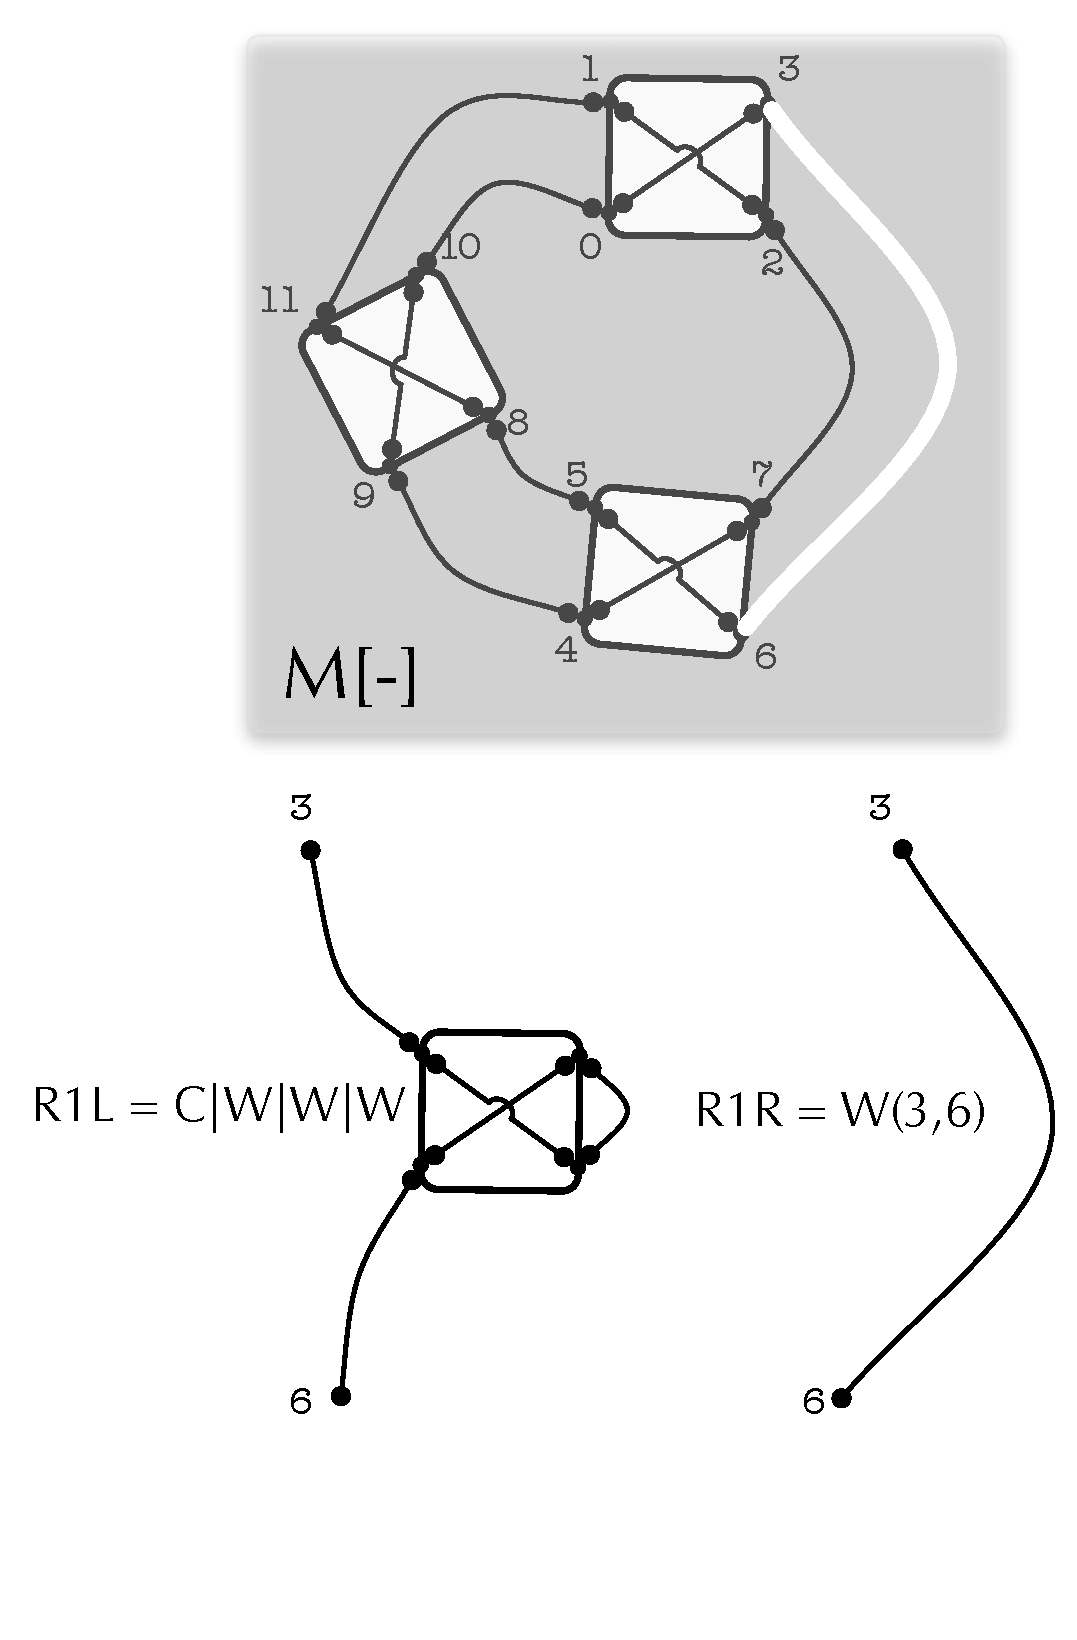
\includegraphics[viewport=30 30 810 550]{../../illustrations/TrefoilContextIllustration}}
    \caption{The figure illustrates a Reidemeister move of the first type as reflected in the context $M$ of the $3_1$  knot, as given in Ex. \ref{example:trefoilcontext}. }
  \label{fig:TrefoilContextIllustration}
\end{figure}
  % The interface of the $R_1$ move is ...
\end{example}

A certain discipline is required in the extended encoding. To
establish our substitution and context lemmas we have to keep the
\textit{interface} (\emph{i.e.} the ports in the process expression
corresponding to the splice points) of the left and right hand sides
of the R-move the same. So, for $R_{1}L$ and $R_{2}L$ we must restrict the ports
that are not the splice points. One way to address this is to embed
the restrictions into the encodings of $R_{1}L$ and $R_{2}L$. Algebraically,

  % \begin{eqnarray}
%     \lefteqn{\meaningof{R_{1}L}(y0,y1) =} \nonumber \\
%     & & (\nu \; x_{0} \; x_{1} \; v_{0} \; v_{1} ) ((\nu \; u)C(x_{0},x_{1},v_{0},v_{1},u) | W(x_{0},x_{1}) | W(y_{0},v_{0}) | W(y_{0},v_{1})) \nonumber \\
%     \lefteqn{\meaningof{R_{2}L}(x_{00},x_{01},x_{10},x_{11}) =} \nonumber \\
%     & & (\nu \; y_{00},y_{01},y_{10},y_{11},)((\nu \; u_{0})C(x_{00},x_{01},y_{00},y_{01},u{0}) \nonumber \\
%     & & | W(y_{00},y_{11}) | W(y_{01},y_{10}) | (\nu \; u_{1})C(x_{10},x_{11},y_{10},y_{11},u_1)) \nonumber
%   \end{eqnarray}

\begin{align*}
  \meaningof{R_{1}L}(y0,y1) = & \\
  (\nu \; x_{0} \; x_{1} \; w_{0} \; w_{1} ) & (W(y_{0},w_{0}) \\
  & |(\nu \; u)C(x_{0},x_{1},w_{0},w_{1},u) | W(x_{0},x_{1}) \\
  & | W(y_{1},w_{1})) \\
  \meaningof{R_{2}L}(x_{00},x_{01},x_{10},x_{11}) = & \\
  (\nu \; y_{00},y_{01},y_{10},y_{11},w_{00},w_{01},w_{10},w_{11}) & (W(x_{00},w_{00}) | W(x_{01},w_{01}) \\
  & | (\nu \; u_{0})C(w_{00},w_{01},y_{00},y_{01},u{0}) \\
  & | W(y_{00},y_{11}) | W(y_{01},y_{10}) \\
  & | (\nu \; u_{1})C(w_{10},w_{11},y_{10},y_{11},u_1) \\
  & | W(x_{10},w_{10}) | W(x_{11},w_{11}))
\end{align*}

  Keeping to the notion of equivalence outlined in the section above,
  however, it will be convenient to factor out the restrictions as in
  the example above.

\begin{figure}[tbp]
%  \centering
 % \scalebox{0.35}[0.350]{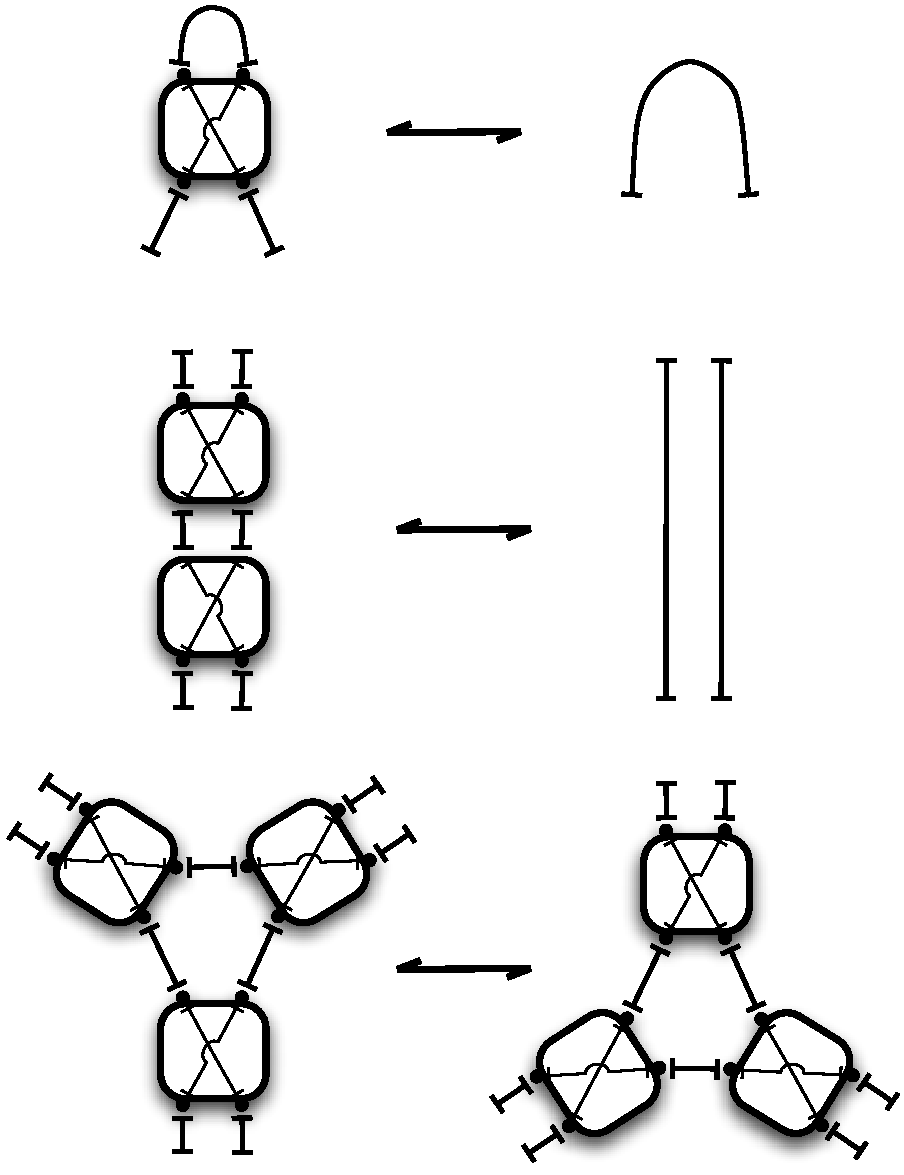
\includegraphics[viewport=30 30 810 550]{../../illustrations/ReidemeisterMovesAsCircuits071115.pdf}}
% Reidemeistermovesascircuits21072006

\center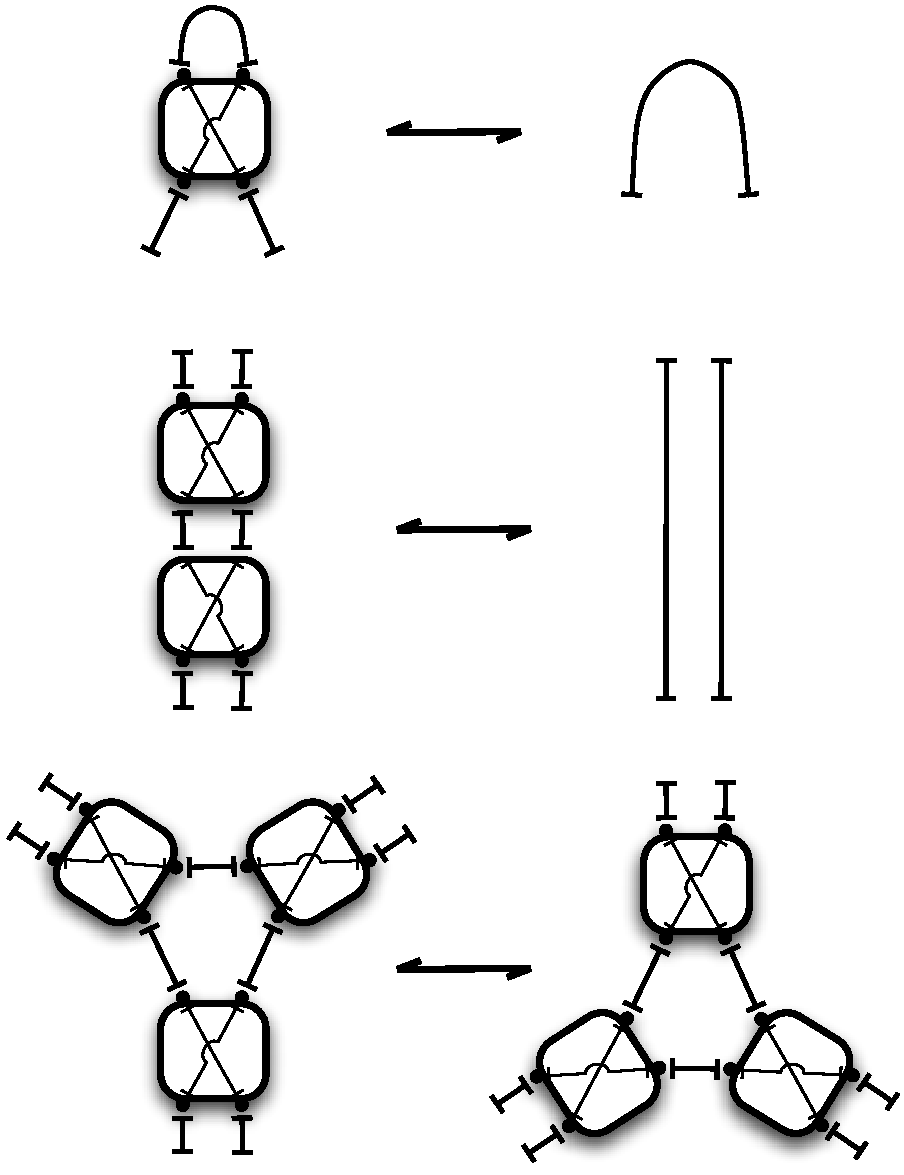
\includegraphics[width=3in]{../../illustrations/ReidemeisterMovesAsCircuits071115.pdf}  
\caption{ Reidemeister moves as bisimilarity-preserving transformations. Cf. Fig. \ref{fig:RMoves}}

\label{fig:RMovesAsXforms}
\end{figure}

\begin{lemma}[context]
$\forall i \in \{ 1, 2, 3 \}$ if $K_{1} \stackrel{R_{i}}{\rightarrow}
K_{2}$ then there exists a context $M$ and (possibly empty) vector of
distinct names $\vec{w}$ such that
  \begin{eqnarray}
    (\nu \; \vec{w})\meaningof{K_{1}}\langle v:w\rangle & = & (\nu \; \vec{w})M[ \meaningof{R_{i}L} ] \nonumber \\
    \meaningof{K_{2}} & = & M[ \meaningof{R_{i}R} ] \nonumber
  \end{eqnarray}
\label{context}
\end{lemma}

\begin{proof}
  This follows directly from the definition of the encoding.
\end{proof}

\begin{lemma}[substitution]
  For all $i \in \{ 1, 2, 3 \}$ $R_{i}L$ is bisimilar to $R_{i}R$ in the
  context of a live encoding. That is, if
  \begin{itemize}
    \item $\meaningof{K} | initSignal$ is alive, and
    \item $\meaningof{K} | initSignal = M[ \meaningof{R_{i}L} ]$
  \end{itemize}
for some context $M$ then we can substitute $\meaningof{R_{i}R}$ in
  its place without change of behavior, i.e.
  \begin{eqnarray}
    (\nu \; \vec{w})M[ \meaningof{R_{i}L} ] & \simeq & M[ \meaningof{R_{i}R} ] \; ,\ \forall i \in \{ 1, 2, 3 \} \nonumber
  \end{eqnarray}
\end{lemma}

\begin{proof}
  This follows from the definitions of $\meaningof{R_{i}\{L,R\}}$ plus
  the requirement that $M$ derives from a live encoding. Even if one
  side has additional synchronizations, there is always enough signal
  to overcome spurious blocking.
\end{proof}

An immediate consequence of these two lemmas is 

\begin{lemma}[1-step]
  if $K_{1}$ can be derived from $K_{2}$ by application of one Reidemeister move, then 

  \begin{eqnarray}
    \meaningof{K_{1}}\langle v \rangle & \simeq & (\nu \; w)\meaningof{K_{2}}\langle v:w \rangle \nonumber
  \end{eqnarray}
\end{lemma}

We are almost in a position to complete the proof of the forward
implication. The next step is to show that you can iterate the
performance of these bisimilarity-preserving transformations in a way
that precisely mimics iterated application of Reidemeister
moves. Because the moves $R_{1}$ and $R_{2}$ change the number of
crossings the number of ports in the interface of the (encoding of
the) knot to which they are applied changes. This is the core issue in
the formal statement of the theorem. Because the splice interface
remains constant across the two sides of a Reidemeister move all one
has to do is keep track of the ports to be hidden. The complete proof
uses a case analysis of the composition of any two types of
Reidemeister moves. We illustrate the analysis in the case of a
simplifying (crossing-elimination) $R_1$ step followed by a complicating
(crossing-introducing) $R_2$ step.

\begin{itemize}
   \item The $R_{1}L$ $\to$ $R_{1}R$ step means we have a context $M$ such that
     \begin{eqnarray}
       (\nu \; x_0 \; x_1 \; w_0 \; w_1)\lefteqn{\meaningof{K_{1}}\langle \vec{v_0}:x_0 : x_1 : w_0 : w_1\rangle} \nonumber \\
       & & = (\nu \; x_0 \; x_1 \; w_0 \; w_1)M[ \meaningof{R_{1}L} ] \nonumber \\
       & & \simeq M[ \meaningof{R_{1}R} ] \nonumber \\
       & & = \meaningof{K_{2}}\langle \vec{v_0} \rangle. \nonumber
     \end{eqnarray}
   \end{itemize}

   \begin{itemize}
   \item The  $R_{2}R$ $\to$ $R_{2}L$ step means we have a context $M'$ such that
     \begin{eqnarray}
       (\nu \; y_{00} \ldots y_{11} \; w_{00} \ldots w_{11})\lefteqn{\meaningof{K_{3}}\langle \vec{v_1}:y_{00}:\ldots : y_{11} : w_{00} : \ldots : w_{11} \rangle} \nonumber \\
       & & = (\nu \; y_{00} \ldots y_{11} \; w_{00} \ldots w_{11})M'[ \meaningof{R_{2}L} ] \nonumber \\
       & & \simeq M'[ \meaningof{R_{1}R} ] \nonumber \\
       & & = \meaningof{K_{2}}\langle \vec{v_1} \rangle. \nonumber
     \end{eqnarray}
   \end{itemize}

\begin{itemize}
     \item Since $\vec{v_0}, \vec{v_1}$ are just lists of distinct names with
      $|\vec{v_0}| = |\meaningof{K_{2}}| = |\vec{v_1}|$, just pick $\vec{v_0} = \vec{v_1}$. Dropping the subscript, we conclude 
     \begin{eqnarray}
       \lefteqn{(\nu \; x_0 \; x_1 \; w_0 \; w_1)\meaningof{K_{1}}\langle \vec{v}:x_0 : x_1 : w_0 : w_1 \rangle \simeq} \nonumber \\
       & & (\nu \; y_{00} \ldots y_{11} \; w_{00} \ldots w_{11})\meaningof{K_{3}}\langle \vec{v_1}:y_{00}:\ldots : y_{11} : w_{00} : \ldots : w_{11} \rangle \nonumber
     \end{eqnarray}
     \item Moreover, we have  $\meaningof{K_{2}}\langle \vec{v} \rangle$ forming the shared core.
   % \item hence $x_0,x_1$ do not occur free in $\vec{v}:y_{00} : y_{01} : y_{10} : y_{11}$,
%      and $y_{00}, y_{01}, y_{10}, y_{11}$ do not occur free in $\vec{v}:x_0 : x_1$
%    \item applying scope extrusion, twice, therefore yields the desired result.
   \end{itemize}

\subsection{Reverse direction. $ K_1 \sim K_2  \Leftarrow  \meaningof{K_1} \simeq \meaningof{K_2}$}

We prove this by contradiction,
assuming two knots in distinct isotopy classes with bisimilar images
and arriving at absurdity. Not surprisingly, the argument in this
direction is considerably less complicated as it is nonconstructive.

Without loss of generality (by application of the lemmas of the forward direction as needed), we assume knots are given in minimal
crossing diagrams. Due to this minimality, if the crossing
numbers of these diagrams are different, then the number of free names (or arity of the
abstractions interpreting the knots)  in  $\meaningof{K_1}$  differs from those  in $\meaningof{K_2}$ --contradicting
bisimilarity. Thus, the crossing numbers must be the same. 

Now we employ the form of the encoding: $\Pi_{i=0}^{n-1}
\meaningof{C(i)}(...) | \Pi_{i=0}^{n-1} W(...)|W(...) \simeq
\Pi_{j=0}^{n-1} \meaningof{C(j)}(...) | \Pi_{j=0}^{n-1}
W'(...)|W'(...)$. Notice that a consequence of sharing the same
crossing number is that the crossing process part of the two encodings
is \emph{identical}. Because bisimulation is a congruence this implies
$\Pi_{i=0}^{n-1} W(...)|W(...) \simeq \Pi_{j=0}^{n-1}
W'(...)|W'(...)$. This says that the only difference can be in the
``wiring harnesses''. Obviously, if any of these wires differ (up to $\alpha$-equivalence), then there
is a  distinguishing barb, contradicting our assumption of
bisimulation.  Hence none of the wires differ, their respective sets of crossings are wired
identically, which means the diagrams are identical. Thus, the knots are ambiently isotopic -- a contradiction.

%\subsection{Strengthening the statement of the theorem}
%
%Let
%  
%   \begin{eqnarray}
%     \lefteqn{L_C(\meaningof{K}\langle \vec{u} \rangle, \vec{v}) :=} \nonumber \\
%     & & \{ (\nu \; u)C(\vec{z}) : \exists P \; \meaningof{K}\langle \vec{u} \rangle = (\nu \; u)C(\vec{z}) | P \} \nonumber \\
%     \lefteqn{L_W(\meaningof{K}\langle \vec{u} \rangle, \vec{v}, \vec{w}) :=} \nonumber \\
%     & & \{ W(a,b) : \exists P \; \meaningof{K}\langle \vec{u} \rangle = W(a,b) | P, a,b \in \vec{v}, a, b \not\in \vec{w} \} \nonumber \\
%     \lefteqn{L(\meaningof{K}\langle \vec{u} \rangle, \vec{v}, \vec{w}) :=} \nonumber \\
%     & & \Pi_{C \in L_{c}(\meaningof{K}\langle \vec{u} \rangle, \vec{v})}C | \Pi_{W \in L_{W}(\meaningof{K}\langle \vec{u} \rangle, \vec{v}, \vec{w})} W \nonumber
%   \end{eqnarray}
%
%   we also have
%
%   \begin{eqnarray}
%     L(\meaningof{K_{1}}\langle \vec{v}:\vec{w_1} \rangle,\vec{v},\vec{w_1}:\vec{w_2}) = L(\meaningof{K_{2}}\langle \vec{v}:\vec{w_2} \rangle,\vec{v},\vec{w_1}:\vec{w_2}) \nonumber
%   \end{eqnarray}
%
%  \begin{itemize}
%  \item When the knots are ambient isotopic the encodings
%    \textit{share} a set of crossings and wires at least as big as a
%    minimal crossing representative of the isotopy class.
%  \item And the other parts are R-move complications of wires that
%    would complete the knot from shared core -- hidden under restriction.
%  \end{itemize}

% section proof sketch (end)

%\section{Unlikely characters: spatial logic for
  knots}\label{sub:characteristic_formulae} % (fold)

Associated to the mobile process calculi are a family of logics known
as the Hennessy-Milner logics. These logics typically enjoy a
semantics interpreting formulae as sets of processes that when
factored through the encoding outlined above allows an identification
of classes of knots with logical formulae. In the context of this
encoding the sub-family known as the spatial logics \cite{CairesC03}
\cite{CairesC04} \cite{Caires04} are of particular interest providing
several important features for expressing and reasoning about
properties (i.e. classes) of knots. We hint here at how this may be done.

%\begin{description}
%\item [structural connectives] 
\subsubsection{Structural connectives} The spatial logics enjoy
structural connectives corresponding, at the logical level, to the
parallel composition ($P | Q$) and new name ($(\nu \; x)P$)
connectives for processes. As illustrated in the examples below, these
connectives are extremely expressive given the shape of our encoding.
%\item [decideable satisfaction]

\subsubsection{Decideable satisfaction}
In \cite{Caires04} the satisfaction relation is shown to be decideable
for a rich class of processes. It further turns out that the image of
the our encoding is a proper subset of that class. This result
provides the basis for an algorithm by which to search for knots
enjoying a given property.
%\item [characteristic formulae]

\subsubsection{Characteristic formulae}
In the same paper \cite{Caires04} , Caires presents a means of calculating
characteristic formulae, selecting equivalence classes of processes
up to a pre--specified depth limit on the support set of names. Composed with our
encoding, this characteristic formula can be used to select
characteristic formulae for knots.
%\end{description}

\subsubsection{Spatial logic formulae}

The grammar below (segmented for comprehension) summarizes the syntax
of spatial logic formulae. We employ illustrative examples in the
sequel to provide an intuitive understanding of their meaning
referring the reader to \cite{Caires04} for a more detailed explication
of the semantics.

\begin{mathpar}
  \inferrule* [lab=boolean] {} {{A,B} \bc T \;|\; \neg A \;|\; A \wedge B \;|\; \eta = \eta'}
  \and
  \inferrule* [lab=spatial] {} {|\; \pzero \;|\; A | B \;|\; x \text{\textregistered} A \;|\; \forall x . A \;|\;  H x . A}
  \and
  \inferrule* [lab=behavioral] {} {|\; \alpha . A}
  \and 
  \inferrule* [lab=recursion] {} {|\; X(\vec{u}) \;|\; \mu X(\vec{u}) . A}
  \and
  \inferrule* [lab=action] {} {\alpha \bc \langle x?(\vec{y}) \rangle \;|\; \langle x!(\vec{y}) \rangle \;|\; \langle \tau \rangle}
  \and 
  \inferrule* [lab=name] {} {\eta \bc x \;|\; \tau}
\end{mathpar} 

% subsection characteristic_formulae (end)   	 

\subsection{Example formulae}\label{sub:example_formulae_} % (fold)

\subsubsection{Crossing as formula.}
% 
% \begin{align*}
%   \frac{d}{dx} \sin x &= \cos x 
%   & \frac{d}{dx} e^x &= e^x \\
%   \frac{d}{dx} \cos x &= - \sin x 
%   & \frac{d}{dx} \log x &= \frac{1}{x} \\
% \end{align*} 

\begin{align*}
 \mu C(x_{0},x_{1},y_{0},y_{1},u).&(\langle x_{0}?(z) \rangle(\langle u! \rangle\langle y_{1}!z \rangle C(x_{0},x_{1},y_{0},y_{1},u)) & \\
  & \wedge \langle y_{1}?(z) \rangle (\langle u! \rangle \langle x_{0}!z \rangle C(x_{0},x_{1},y_{0},y_{1},u)) & \\
  & \wedge \langle x_{1}?(z) \rangle (\langle u? \rangle \langle y_{0}!z \rangle C(x_{0},x_{1},y_{0},y_{1},u)) & \\
  & \wedge \langle y_{0}?(z) \rangle (\langle u? \rangle \langle x_{1}!z \rangle C(x_{0},x_{1},y_{0},y_{1},u))) &
\end{align*}

The lexicographical similarity between the shape of this formulae and
the shape of definition of the process representing a crossing reveals
the intuitive meaning of this formulae. It describes the capabilities
of a process that has the right to represent a crossing. For example
it picks out processes that may perform an input on the port $x_0$ in
its initial menu of capabilities. What differentiates the formula
from the process, however, is that the crossing process is the
smallest candidate to satisfy the formula. Infinitely many other
processes -- with internal behavior hidden behind this interface, so
to speak -- also satisfy this formula. Even this simple formula,
then, can be seen to open a new view onto knots, providing a
computational interpretation of \emph{virtual} knots.

Note that this formula is derived by hand. A similar formula can be
derived by employing Caires' calculation of characteristic formula
\cite{Caires04} to the process representing a crossing. In light of
this discussion, we let
$\meaningof{C}_{\phi}(x0,x1,y0,y1,u)$ denote a formula specifying the
dynamics we wish to capture of a crossing. To guarantee we preserve
the shape of the interface and minimal semantics we demand that
$\meaningof{C}_{\phi}(x0,x1,y0,y1,u) \Rightarrow
\textbf{C}(x0,x1,y0,y1,u)$ where $\textbf{C}(x0,x1,y0,y1,u)$ denotes
the formula above.
                            
\subsubsection{Crossing number constraints.}
The moral content of the context lemma (Lemma \ref{context}) is that the notion of
``locality'' in the Reidemeister moves is effectively captured by the
parallel composition operator of the process calculus. This intuition
extends through the logic. Given a formula,
$\meaningof{C}_{\phi}(x0,x1,y0,y1,u)$, we can use the structural
connectives to specify constraints on crossing numbers, such as at
least $n$ crossings, or exactly $n$ crossings.
\begin{mathpar}
  \inferrule* [lab=at-least-n] {} { K^{\geq n}_{\phi}(\vec{xs},\vec{ys}) := \Pi_{i=0}^{n-1} Hu . \meaningof{C}_{\phi}(xs_i,ys_i,u) | T }
  \and 
  \inferrule* [lab=exactly-n] {} { K^{= n}_{\phi}(\vec{xs},\vec{ys}) := \Pi_{i=0}^{n-1} Hu . \meaningof{C}_{\phi}(xs_i,ys_i,u) | \neg (\forall x_0,y_0,x_1,y_1,u . \meaningof{C}_{\phi}(x_0,y_0,x_1,y_1,u) | T) }
\end{mathpar}

To round out this section, recall that the encoding of an $n$-crossing
knot decomposes into a parallel composition of $n$ \emph{copies} of a
crossing process together with a wiring harness. To specify different
knot classes with the same crossing number amounts to specifying
logical constraints on the wiring harness. In the interest of space,
we defer examples to a forthcoming paper. Suffice it to say that both
the conditions ``alternating knot'' and ``contains the tangle
corresponding to 5/3'' are expressible. For example, it is possible to
calculate the characteristic formula of a process corresponding to the
tangle 5/3 and conjoin it into the classifying formula via the
composition connective of the logic.

Finally, we wish to observe that it is entirely within reason to
contemplate a more domain-specific version of spatial logic tailored
to the shape of processes in the image of the encoding. Such a
domain-specific logic would have a better claim to the title formal
language of knot properties.

% subsection example_formulae_ (end)

% section knots_as_processes (end) 

% section spatial logic via knots (end)

\section{Conclusions and future work}

\paragraph{Testing physical space}
You, gentle reader, may wonder why of all the theorems to be proved
given this set up we pick the one above. In some sense it's hardly
central to quantum mechanics. We see it as central in the sense that
it firmly establishes a notion of physical space arising from a notion
of the equivalence of behavior. Relating bisimulation to a metric is a
big step forward, but one is faced with interpreting the relationship
of that metric space to something more physical. Quantum mechanical
notions of ``physical'' space are still far from intuitive, but by
relating this idea of distance as testing to calculations that predict
physical circumstances we are making a not insignificant step forward
toward an understanding of the physical space we inhabit as
essentially dynamic.

\paragraph{Effectivity and simulation}
One of the observations we have yet to make is that the entire program
spelled out here is effective. We have built various interpreters for
the reflective calculus at work in this interpretation. In principle,
then, we can simulate quantum mechanics on a computer. The place where
the simulation may lose fidelity is the infinitely branching summation
for the annihilator.

In this connection i also want to point out that the evaluation style
calculation of the inner product puts the non-determinism of the
summation right at the heart of measurement. This suggests that
Milner's original reduction-based formulation of the dynamics of his
calculi in terms of sums was not just notationally suggestive of a
notion of measure-and-continue but captured some significant part of
the physics.

\paragraph{Quantum continuations}
In light of this last observation i want to point out that the
predominant account of quantum mechanics is missing a key aspect of a
truly compositional story of the physical situation. In a real lab,
when a measurement is made the observation can be made to feed into
another device that then makes another measurement conditioned on the
results of the first. This means that after the superposition was
collapsed the entire experimental set up remained in
superposition. While QM offers a means of writing this down it doesn't
quite line up well with the well-trodden formulation of computation
and continuation that we see so succinctly expressed in Milner's
calculi. This suggests that there might be advantages to this account
of dynamics waiting to be explored.

\paragraph{Quantum logic}
In this connection, we also note that by virtue of having the
Hennessy-Milner construction, we can pull the construction through the
interpretation of QM. This gives us a natural candidate for a quantum
logic that enjoys an extremely tight connection with it's domain of
interpretation, making the construction much less ad hoc (rather it is
the image of functor!).

\paragraph{Quantum probabiity}
i have questions about the basis of the interpretation of inner
product as probability amplitude. In particular, using which
axiomatization of probability theory does the notion of probability
amplitude earn the right to be so dubbed? In other words, where is the
proof that the operation for calculating a probability amplitude (and
then squaring) satisfies the axioms of what it means to calculate a
probability? Even if such a proof exists (i have yet to find it in the
literature), i wonder if it might not be possible to turn things on
their heads. Can we view the calculation of the probability amplitude
as an axiomatization of probability? If so, then the definition we
give for calculating probability amplitude may provide the basis for
an \emph{effective} theory of probability.

\paragraph{Quantum vs ``biological'' information}
Finally, i want to conclude with a more philosophical observation. At
a recent workshop in which QM was a predominant topic i noticed
something about quantum information. The speaker was giving a riveting
discussion of axiomatic QM and showing how properties of ``no
cloning'' and ``no deleting'' emerged as consequences of the
axiomatization. Theorems of this form are necessary to give us a sense
of confidence that our axioms characterize the physical theory. What
struck me, though, was that if quantum information is neither erasable
nor replicable it is markedly different from \emph{life}. Two of the
things we know about life is that

\begin{itemize}
  \item it ends;
  \item to gain some measure of persistence, to transcend it's
    finitude it is imminently copyable.
\end{itemize}

Both of these qualities are summarized succinctly in the aphorism: all
flesh is grass. For me these two kinds of ``information'' -- call them
quantum and biological -- are end points on a spectrum of strategies
for persistence. At one end, we have those curious entities that enjoy
uniqueness and permanence; at the other, we have those who in the face
of a certain end and an uncertain present make a go of passing
something on. To me one of the more remarkable aspects of the latter
strategy is that in the presence of noise (and certain features of
copying) we get a kind of dynamism, a chance for improvement against a
given persistent condition.

% subsection other_calculi_other_bisimulations_and_geometry_as_behavior (end)




% section conclusion (end)

%\section{Appendix: From DT-codes to processes}

What follows is an algorithm for calculating the $\omega$ indexing
function. Note that the function \emph{over} can be implemented easily using the function $\delta$, or the function $sgn$, described in section \ref{ssub:dowker_thistlethwaite_codes}. Exercise for the reader: upgrade the algorithm so that wires
are not duplicated during the process.  \newpage

%  \begin{lstlisting}
\begin{verbatim}
(* ------------------------------------------------------------------ *)
(*                                                                    *)
(* Given types Knot and Wire, the omega function is typed as follows  *)
(* omega : int -> (int -> int) -> (int -> int) -> Knot -> (Wire list) *)
(* With dt a table representing the Dowker-Thistlethwaite mapping     *)
(* from odds to evens, and dti the inverse. The function keeps an     *)
(* accumulator, acc, in which to collect the wires it calculates.     *)
(* The function assumes helper functions C and x0,x1,y0,y1. C takes   *)
(* and instance of type Knot and the odd index of the DT code and     *)
(* returns the crossing. The other helpers are accessors of the ports *)
(* of the crossing. The algorithm visits every crossing and so        *)
(* generates many wires more than once, which is why the accumulator  *)
(* is updated with union rather than cons on the recursive calls. As  *)
(* an exercise, modify the algorithm to avoid wire duplication.       *)
(*                                                                    *)
(* ------------------------------------------------------------------ *)

let omega i dt dti knot acc = 
  if (i <= (numCrossings knot)) 
     then 
       let ic = (2*i - 1) in 
         (omega 
            (i+1) dt dti knot 
            (union acc 
               [ W(x1(C(knot,ic)), 
                 (if (over dt ic-1)
                     then y0(C(knot,ic-1))
                     else y1(C(knot,ic-1)))); 
                 W(y0(C(knot,ic)), 
                 (if (over dt ic+1)
                     then x1(C(knot,ic+1))
                     else x0(C(knot,ic+1)))); 
                 W(x0(C(knot,ic)), 
                 (if (over dt (dti ((dt ic)-1)))
                     then y0(C(knot,(dti ((dt ic)-1))))
                     else y1(C(knot,(dti ((dt ic)-1)))))); 
                 W(y1(C(knot,ic)), 
                 (if (over dt (dti ((dt ic)+1)))
                     then x1(C(knot,(dti ((dt ic)+1))))
                     else x0(C(knot,(dti ((dt ic)+1)))))) ])) 
     else acc
\end{verbatim}
%     \end{lstlisting}

%%% Local Variables:
%%% Tex Master:"jktir.tex"
%%% End: 

% section wiring algorithm (end)

\paragraph{Acknowledgments.}
The author wishes to thank Phil Scott for bringing the
normalization-by-evaluation program to his attention. It turned out to
be a key piece of the puzzle.
 

% section acknowledgments (end)

\newpage


\bibliographystyle{plain}   
\bibliography{../../biblios/main.bib}

\section{Appendix :  reflection in more detail}\label{appendix:rho_details}

\subsection{Name equivalence}

We now come to one of the first real subtleties of this calculus as
compared to other process calculi. Both the calculation of the free
names of a process and the determination of structural congruence
between processes critically depend on being able to establish whether
two names are equal. In the case of the calculation of the free names
of an input-guarded process, for example, to remove the bound name we
must determine whether it is in the set of free names of the
continuation. Likewise, structural congruence includes
$\alpha$-equivalence. But, establishing $\alpha$-equivalence between
the processes $x?(z).\lift{w}{y!(z)}$ and $x?(v).\lift{w}{y!(v)}$, for
instance, requires calculating a substitution,
e.g. $x?(v).\lift{w}{y!(v)}\{z / v \}$. But this calculation requires,
in turn, being able to determine whether two names, in this case the
name in the object position of the output, and the name being
substituted for, are equal.

As will be seen, the equality on names involves structural equivalence
on processes, which in turn involves alpha equivalence, which involves
name equivalence. This is a subtle mutual recursion, but one that
turns out to be well-founded. Before presenting the technical details,
the reader may note that the grammar above enforces a strict
alternation between quotes and process constructors. Each question
about a process that involves a question about names may in turn
involve a question about processes, but the names in the processes the
next level down, as it were, are under fewer quotes. To put it another
way, each `recursive call' to name equivalence will involve one less
level of quoting, ultimately bottoming out in the quoted zero process.

Let us assume that we have an account of (syntactic) substitution and
$\alpha$-equivalence upon which we can rely to formulate a notion of
name equivalence, and then bootstrap our notions of substitution and
$\alpha$-equivalence from that. We take name equivalence, written
$\nameeq$, to be the smallest equivalence relation generated by the
following rules.

\begin{mathpar}
\inferrule*[left=Quote-drop]
{ }
{ \quotep{\dropn{x}} \nameeq x }

\inferrule*[right=Struct-equiv]
{ P \scong Q }
{ \quotep{P} \nameeq \quotep{Q} }
\end{mathpar}

\subsection{Syntactic substitution}

Now we build the substitution used by $\alpha$-equivalence. We use
$\Proc$ for the set of processes, $\QProc$ for the set of names, and
$\id{\{}\vec{y} / \vec{x} \id{\}}$ to denote partial maps, $s : \QProc
\rightarrow \QProc$. A map, $s$ lifts, uniquely, to a map on process
terms, $\widehat{s} : \Proc \rightarrow \Proc$ by the following
equations.

\begin{mathpar}
(0) \psubstp{Q}{P}         :=    0 \\
(R \juxtap S) \psubstp{Q}{P}
		:=    
		(R)\psubstp{Q}{P} \juxtap (S) \psubstp{Q}{P} \\
(x?(y).R) \psubstp{Q}{P}    
		:=    
		(x)\substp{Q}{P} (z)\concat( (R \psubstn{z}{y}) \psubstp{Q}{P} ) \\
(\lift{x}{R}) \psubstp{Q}{P}  
 		:=
 		\lift{(x)\substp{Q}{P}}{ R \psubstp{Q}{P} } \\
(\dropn{x})  \psubstp{Q}{P}       
		:= 
		\left\{ 
			\begin{array}{ccc} 
				\dropn{\quotep{Q}} & & x \nameeq \quotep{P} \\
                              	\dropn{x} & & otherwise \\
			\end{array}
		\right. 
\end{mathpar}
 

where

\begin{eqnarray}
(x)\id{\{} \lpquote Q \rpquote / \lpquote P \rpquote \id{\}}            = 
		\left\{ 
			\begin{array}{ccc}
				\lpquote Q \rpquote & & x \nameeq \lpquote P \rpquote \\
                                x & & otherwise \\
			\end{array}
		\right. \nonumber
\end{eqnarray}

and $z$ is chosen distinct from $\quotep{P}$, $\quotep{Q}$, the free
names in $Q$, and all the names in $R$. Our $\alpha$-equivalence will
be built in the standard way from this substitution.

But, given these mutual recursions, the question is whether the calculation
of $\nameeq$ (respectively, $\scong$, $\alphaeq$) terminates. To
answer this question it suffices to formalize our intuitions regarding
level of quotes, or quote depth, $\#(x)$, of a name $x$ as
follows.

\begin{eqnarray}
	\#(\quotep{P}) & = & 1 + \#(P) \nonumber\\
    \#(P) & = & \left\{
			   \begin{array}{ccc}
				 max\{ \#(x) : x \in \names{P} \} & & \names{P} \neq \emptyset \\
				 0 & & otherwise \\
			   \end{array}
			\right. \nonumber
\end{eqnarray}

The grammar ensures that $\#(\quotep{P})$ is bounded. Then the
termination of $\nameeq$ (respectively, $\scong$, $\alphaeq$) is an
easy induction on quote depth.

\begin{remark}
  Note that by a related piece of reasoning we can see that $\forall
  P. \quotep{P} \not\in \freenames{P}$.
\end{remark}

\subsection{Semantic substitution}

The substitution used in $\alpha$-equivalence is really only a device
to formally recognize that binding occurrences do not depend on the
specific names. It is not the engine of computation. The proposal here
is that while synchronization is the driver of that engine, the real
engine of computation is a semantic notion of substitution that
recognizes that a dropped name is a request to run a process. Which
process? Why the one whose code has been bound to the name being
dropped. Formally, this amounts to a notion of substitution that
differs from syntactic substitution in its application to a dropped
name.

\begin{eqnarray}
(\dropn{x})  \psubstp{Q}{P}       
		& = & 
		\left\{ 
			\begin{array}{ccc} 
				Q & & x \nameeq \quotep{P} \\
                              	\dropn{x} & & otherwise \\
			\end{array}
		\right. \nonumber
\end{eqnarray}

In the remainder of the paper we will refer to semantic and syntactic
substitutions simply as substitutions and rely on context to
distinguish which is meant. Similarly, we will abuse notation and
write $\substn{y}{x}$ for $\psubstn{y}{x}$.



\end{document}

